
%%%%%%%%%%%%%%%%%%%%%%%%%%%%%%%%%%%%%%%%%%%%%%%%%%%%%%%%%%%%%%%%%%%%%%%%%%%%%%%%
%%%%%%%%%%%%%%%%%%%%%%%%%%%%%%%%%%%%%%%%%%%%%%%%%%%%%%%%%%%%%%%%%%%%%%%%%%%%%%%%
\section{Definições relativas as danças a dois}

Antes de iniciar as explicações no capítulo, 
é necessário partir desde uma linguagem comum;
com este propósito, 
significados de algumas palavras bem definidas na literatura são mostrados a continuação:
 
\begin{definition}[Princípio:] 
\index{Princípios}
\label{def:Principio}O Dicionário Priberam da Língua Portuguesa \cite{priberamprincipio} define princípio como:
Frase ou raciocínio que é base de uma arte, de uma ciência ou de uma teoria.
Adicionalmente o Dicionário Online de Português, DICIO \cite{dicioprincipio}, define princípio como:
Informação básica e necessária que fundamenta uma seção de conhecimentos.
Exemplo: Princípios da matemática.
\end{definition}

\begin{definition}[Casal:] 
\index{Casal}
\label{def:Casal} O Dicionário Priberam da Língua Portuguesa \cite{priberamcasal} define casal como:
Par formado por um macho e uma fêmea.
Exemplo: casal de cavalos, casal de pombas, casal de humanos.
\end{definition}

\begin{definition}[Par:] 
\index{Par}
\label{def:Par} O Dicionário Priberam da Língua Portuguesa \cite{priberampar} define par como:
Igual, semelhante, parceiro.
Cada uma das pessoas que constituem uma dupla na dança.
\end{definition}


%%%%%%%%%%%%%%%%%%%%%%%%%%%%%%%%%%%%%%%%%%%%%%%%%%%%%%%%%%%%%%%%%%%%%%%%%%%%%%%%
\subsection{Definições sobre condução nas danças a dois}
Usando como base os significados mostrados anteriormente, 
serão descritos alguns termos muito utilizados tradicionalmente na dança\footnote{
Para as definições, foi priorizado o uso da palavra par sobre a palavra casal,
para poder definir às entidades dançantes independentemente do sexo dos participantes.}.
Assim,  são propostas as seguintes definições:

\begin{definition}[Paradigma da condução (Dança):] 
\index{Condução} 
\label{def:ParadigmaConducao} 
Este é um modelo de dança usado na \hyperref[def:DancaSalao]{\textbf{dança de salão}},
\hyperref[def:DancaSocial]{\textbf{dança social}}, etc. 
E indica que entre as pessoas que conformam o \hyperref[def:Par]{\textbf{par}} de dança,
existe uma transmissão de informação relativa à movimentação e as pausas; 
de modo que, a informação tem um fluxo unidirecional no médio de transmissão,
que vá desde um \hyperref[def:Condutor]{\textbf{condutor}} (Transmissor/Tx) 
ate um \hyperref[def:Seguidor]{\textbf{seguidor}} (Receptor/Rx),
ver Figura \ref{fig:paradigmaconducion}. 
\end{definition}
\index{Condutor} 

\begin{figure}[!ht]
     \centering
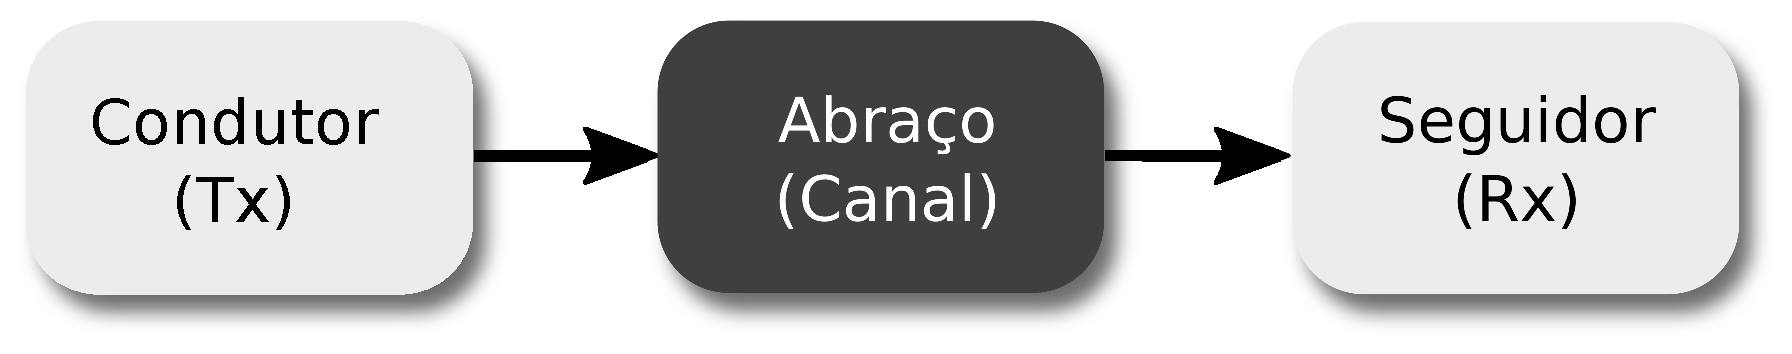
\includegraphics[width=0.75\textwidth]{chapters/cap-normas/modeloconducao.eps}
\caption{Fluxo da informação na condução}
\label{fig:paradigmaconducion}
\end{figure}

Seguindo a desigualdade de processamento de dados (do inglês ``data-processing inequality''),
qualquer processamento efetuado sobre um pacote de informação 
nunca nos proporcionará mais informação da contida no pacote;
é dizer, qualquer processamento da informação só produzirá perdas,
ou num caso ideal obteremos a mesma quantidade de informação  \cite[pp. 34]{cover2006elements}.
Assim, quando utilizamos o \hyperref[def:ParadigmaConducao]{\textbf{paradigma da condução}} na nossa dança,
as transformações efetuadas pelo meio de transmissão (o abraço),
e as subjetividades na interpretação da informação por parte do seguidor, 
só podem produzir perdas sobre a informação transmitida pelo condutor;
assim, devemos ter muito cuidado, no nosso abraço de dança,
procurando a \hyperref[def:brazosfirmes]{\textbf{firmeza de braços}}, 
para que a informação enviada pelo \hyperref[def:Condutor]{\textbf{condutor}} 
chegue ao \hyperref[def:Seguidor]{\textbf{seguidor}} o mais integra possível.

Assim, obter o 100\% de eficiência na transmissão ``bruta'' da informação
é  um alvo teórico possível; porem, pouco provável de acontecer na prática.
Entretanto, é possível atingir valores próximos ao 100\% de eficiência,
se agregamos uma boa quantidade de redundância na informação transmitida na condução \cite[pp. 184,219]{cover2006elements};
é dizer, que para indicar um mesmo movimento ao seguidor devemos enviar mais de uma indicação 
para uma mesma ideia de movimento proposto. Por exemplo, 
além de usar os braços para indicar um movimento, 
poderíamos usar peso de nosso corpo para indicar a direção, inclusive nosso olhar;
sendo esta uma triple redundância.
 

\begin{definition}[Condutor (Dança):] 
\index{Condutor} 
\label{def:Condutor} 
Tradicionalmente se entende como 
condutor à pessoa que tem o papel de conduzir ou propor o movimento ao 
\hyperref[def:Seguidor]{\textbf{seguidor}}. 
O objetivo técnico das pessoas que optam por este rol na dança, é chegar 
a ter a sensibilidade necessária para entender onde está localizado espacialmente, 
e como distribui o peso do corpo, o \hyperref[def:Seguidor]{\textbf{seguidor}}; 
de modo que seja possível para o condutor aplicar sobre o 
\hyperref[def:Seguidor]{\textbf{seguidor}}, 
uma mistura de indicações, forças ou torções,  
para provocar os movimentos ou pausas desejadas;
chama-se a isto saber conduzir.
Sinônimos de condutor: Líder (Dança).
\end{definition}

\begin{definition}[Seguidor (Dança):] 
\index{Seguidor} 
\index{Conduzido} 
\label{def:Seguidor} 
Tradicionalmente se entende como 
seguidor à pessoa que recebe a condução e proporciona uma resposta corporal. 
O objetivo técnico das pessoas que optam por este rol na dança, é chegar 
a ter a sensibilidade necessária para entender e incorporar as conduções,
independentemente de quem seja a pessoa que aplique a condução;
chama-se a isto ser conduzível.
Sinônimos de seguidor: \textbf{Conduzido}.
\end{definition}

O \hyperref[def:ParadigmaConducao]{\textbf{paradigma da condução}},
 descreve tradicionalmente 
um modelo de transmissão unidirecional da informação entre dois pontos
usando um único canal de comunicação;
entretanto, como é visto na Figura \ref{fig:tiposcomunica}, 
na área de estudo das telecomunicações 
sabemos que existem outros modelos de 
transmissão de informação que podem ser explorados 
sobre um único canal de comunicação. 
Nesse sentido 
nos últimos anhos tem surgido diversas novas propostas para o termo ``condução''
e suas subdivisões.
\begin{figure}[!ht]
     \centering
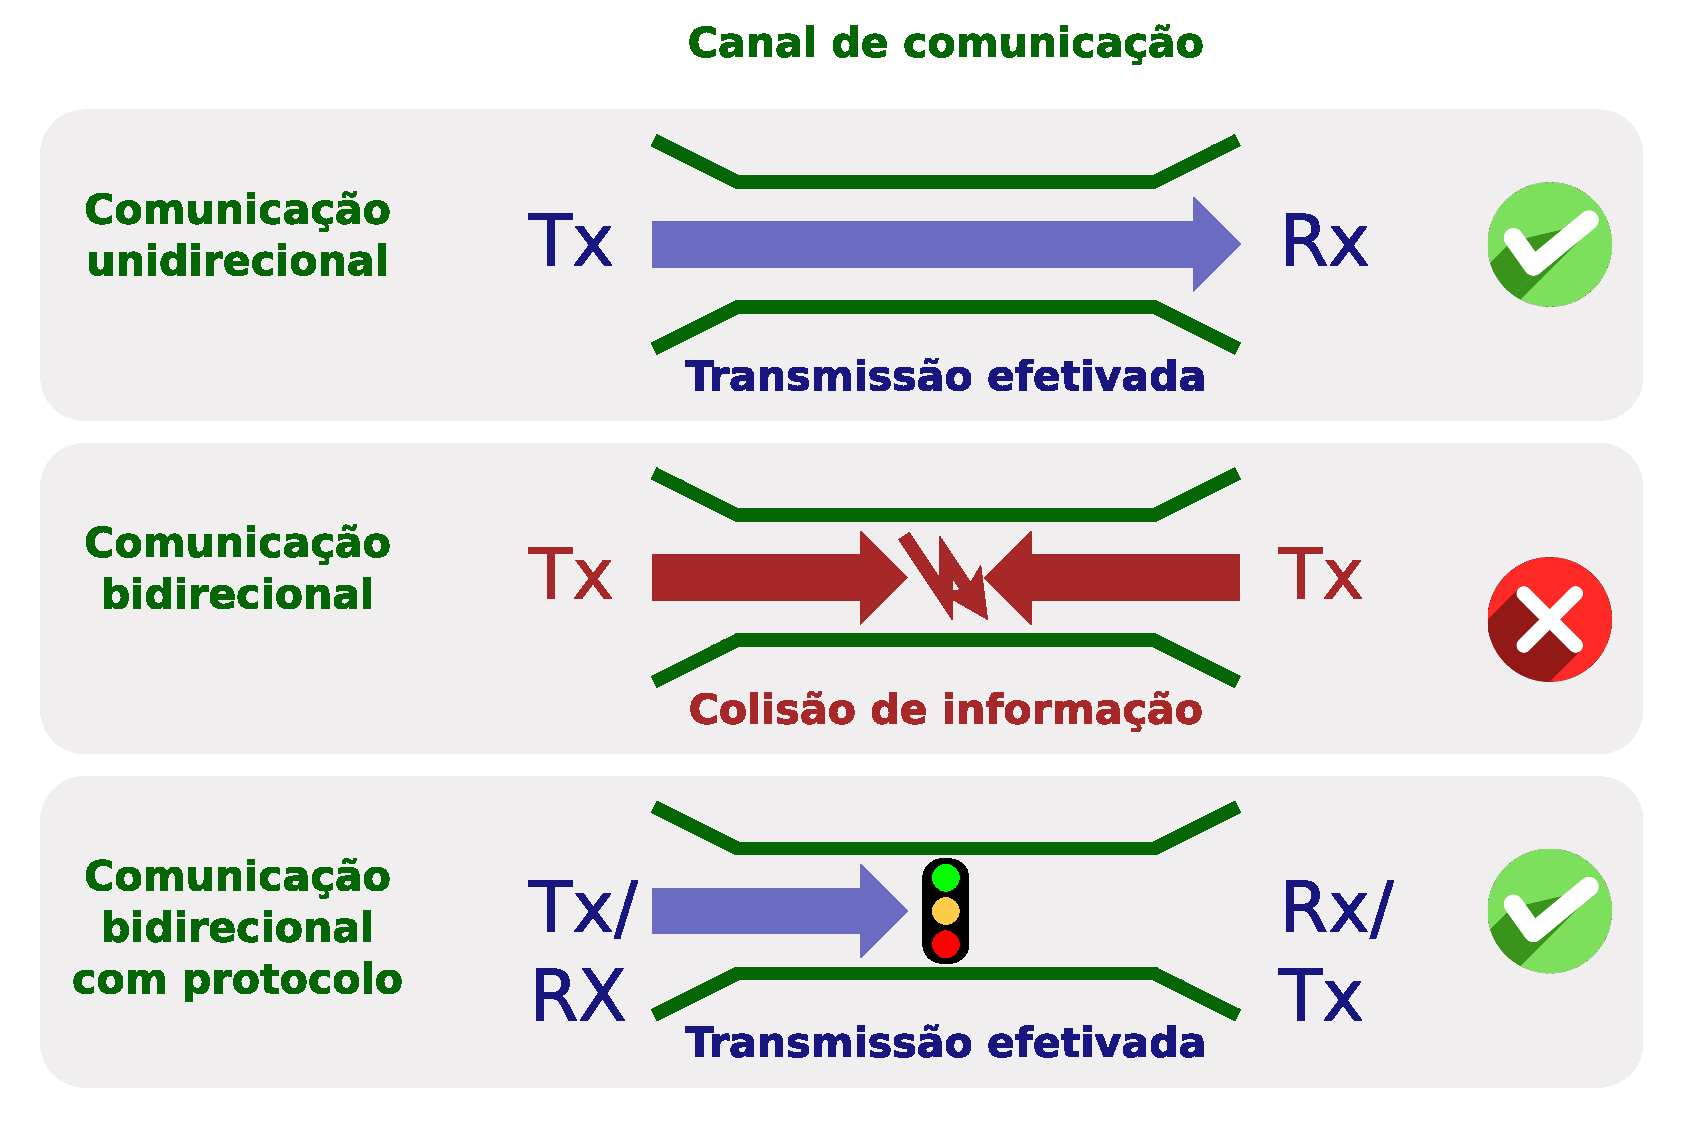
\includegraphics[width=0.95\textwidth]{chapters/cap-normas/tiposcomunica.eps}
\caption{Comunicação unidirecional vs. bidirecional.}
\label{fig:tiposcomunica}
\end{figure}


Vários professores de dança tem proposto ou utilizam diferentes tipos de subdivisões para categorizar
a condução; por exemplo, a ``Universidade de Dança de Salão'' 
coordenada e direcionada pelo professor, correógrafo e dançarino Rodrigo Delano,
organiza e sistematiza o ensino da dança usando dois tipos de 
classificações para a condução;
uma em função do método usado para transmitir informação (tipos de condução) e outra em 
função do fluxo da informação (tipos de relação) no \hyperref[def:Par]{\textbf{par}} de dança.  
\begin{description} 
%%%%%%
\item [Tipos de condução:]  A continuação são listados os tipos de condução em função da mecânica 
ou do método usado para transmitir informação entre o 
\hyperref[def:Par]{\textbf{par}} de dança. 
\begin{itemize}
    %%%%%
    \item \textbf{Condução mãos e braços:} 
    Nesta técnica o \hyperref[def:Condutor]{\textbf{condutor}} 
    usa suas mãos e braços para transmitir 
    ao \hyperref[def:Seguidor]{\textbf{seguidor}} 
    as informações do movimento proposto.
    A condução mãos e braços tende a ser mais eficiente (não quer dizer mais procurada) 
    que a \hyperref[ref:conducaocorporal]{\textbf{condução corporal}}
    na transmissão de informação.
    \item \textbf{Condução corporal:}\label{ref:conducaocorporal}
    Nesta técnica o \hyperref[def:Condutor]{\textbf{condutor}} usa o 
    corpo como um todo para transmitir ao \hyperref[def:Seguidor]{\textbf{seguidor}}
    os detalhes do movimento. 
    Controle e dissociação corporal são temas muito relevantes neste tipo de condução.
    \item \textbf{Condução por indução:} Esta é a condução a distancia 
    (sem contato físico).
    Geralmente é possível ver que este tipo de condução usa o olhar, a postura, 
    e a intenção de movimento do corpo, 
    para transmitir informação ao \hyperref[def:Seguidor]{\textbf{seguidor}}.
\end{itemize}
%%%%%%
\item [Tipos de relação:] A continuação são listados 
os tipos de condução em função da relação do fluxo de informação
entre o \hyperref[def:Par]{\textbf{par}} de dança.
\begin{itemize}
    %%%%%
    \item \textbf{Condução descritiva:} 
    Esta é uma técnica desenvolvida na base da biomecânica corporal,
    o objetivo desta técnica é que o 
    \hyperref[def:Condutor]{\textbf{condutor}} consiga transmitir/descrever 
    todos os detalhes do movimento, mediante o uso de todos seus artifícios de condução,
    de modo que o \hyperref[def:Seguidor]{\textbf{seguidor}} 
    não tenha margem de dúvida sobre o movimento.

    Neste caso o condutor procura utilizar ao máximo o canal de comunicação,
    possivelmente enviando informação com redundância, 
    para garantir que o seguidor receba de forma integra a informação.
    %%%%%
    \item \textbf{Condução proposta:} 
    Neste tipo de condução, o 
    \hyperref[def:Condutor]{\textbf{condutor}} propõe o movimento,
    mas existe uma margem para que o \hyperref[def:Seguidor]{\textbf{seguidor}} 
    finalize ou de acabamento ao movimento proposto (precisa atitude do seguidor).
    Geralmente é possível ver que a maioria das conduções propostas 
    são realizadas mediante uma \hyperref[ref:conducaocorporal]{\textbf{condução corporal}} 
    (marcante transferência de peso e direção no corpo).

    Neste caso o condutor utiliza completamente o canal de comunicação,
    mas não está preocupado na total integridade na recepção da informação enviada,
    pois considera exitosa a transmissão se a informação recebida 
    tem um margem pequeno de erro/mudanças.
    %%%%%
    \item \textbf{Condução com troca de proponência:}
    Neste tipo de condução o \hyperref[def:Condutor]{\textbf{condutor}} 
    deixa um vazio ou silencio na transmissão
    de informação ao \hyperref[def:Seguidor]{\textbf{seguidor}},
    para dar espaço para o seguidor (agora transmissor) 
    propor um movimento, de modo que se seu par estiver receptivo 
    conseguirá continuar este movimento. 


    Neste caso o condutor não utiliza o tempo todo o canal de comunicação,
    deixando pequenos porcentagens de silêncios
    para permitir momentaneamente a inversão do fluxo de informação.
    %%%%%
    \item \textbf{Condução compartilhada:} 
    Neste tipo de condução, existe entre ambos membros do 
    \hyperref[def:Par]{\textbf{par}} de dança, 
    um fluxo continuo de informação, sem colisão, 
    indo em ambos sentidos de forma equilibrada. 
    
    Neste caso o fluxo de informação no canal de comunicação muda continuamente de direção,
    pelo que não se pode estabelecer de forma fixa a figura do condutor ou do seguidor.
    %%%%%
    \item \textbf{Condução mutua:} Neste tipo de fluxo de informação 
    os dois membros do \hyperref[def:Par]{\textbf{par}} de dança 
    transmitem cotidianamente informação, 
    de modo que esta tende a colidir fusionando-se gerando uma informação
    diferente à enviada pelos dois transmissores.
    Neste caso u objetivo principal na dança é a cocriação de movimentos 
    e não a transferência de informação ao par de dança. 
     

\end{itemize}

    Nesta organização e sistematização percebemos que 
    uma pessoa do par de dança não perde o título de condutor mesmo que ele, por alguns poucos
    instantes (falando porcentualmente), deixe de transmitir e passe  
    a receber informação.
    Assim, nesta sistematização a figura do condutor, e consequentemente do seguidor, 
    não é binária e discreta em relação à transmissão e recepção de informação, tendo na verdade 
    cada pessoa vários pontos intermediários e contínuos para a relação transmissão/recepção; 
    de modo que uma pessoa do par de dança só perde o título de condutor quando esta
    deixa maioritariamente de transmitir informação. 
\end{description}
%%%%%%%%%%%%%%%%%%%%%%%%%%%%%%%%%%%%%%%%%%%%%%%%%%%%%%%%%%%%%%%%%%%%%%%%%%%%%%%%
\subsection{Definições sobre tipos de danças a dois}

Nas definições desta seção, foram tomados dois conceitos do artigo 
``Conceitos e definição de Dança de Salão'' \cite{Zamoner2012};
modificações foram feitas para adaptar estas definições aos conceitos de 
\hyperref[def:Condutor]{\textbf{condutor}} e \hyperref[def:Seguidor]{\textbf{seguidor}}, 
usados ao longo deste livro.

\begin{definition}[Dança social:]
\index{Dança social} 
\label{def:DancaSocial} 
É uma dança com fim recreativo de prática social, não cênica, nem competitiva, 
que não tem um interesse artístico, histórico, geográfico ou técnico; 
que se universaliza e consiste na movimentação dos corpos do \hyperref[def:Par]{\textbf{par}} de dança  \cite{Zamoner2012}, 
onde existe o rol do \hyperref[def:Condutor]{\textbf{condutor}} 
e do \hyperref[def:Seguidor]{\textbf{seguidor}} (papeis intercambiáveis), 
ate onde o nível técnico do par o permita.
\end{definition}

\begin{definition}[Dança de salão:]
\index{Dança de salão}
\label{def:DancaSalao}  
É uma arte que procura conservar suas características técnicas, 
sua origem histórica e geográfica, e se universaliza em práticas sociais. 
Esta arte consiste na interpretação improvisada da música por médio dos movimentos 
dos corpos de um \hyperref[def:Par]{\textbf{par}} de dança \cite{Zamoner2012}, 
utilizando o \hyperref[def:ParadigmaConducao]{\textbf{paradigma da condução}} .
\end{definition}

%%%%%%%%%%%%%%%%%%%%%%%%%%%%%%%%%%%%%%%%%%%%%%%%%%%%%%%%%%%%%%%%%%%%%%%%%%%%%%%%
\subsection{Definições sobre as divisões na estrutura anatômica do corpo }
\begin{definition}[Plano axial:] 
\index{Plano axial}
\label{def:PlanoAxial}
O Dicionário Priberam da Língua Portuguesa \cite{priberamplano} define plano axial como:
Plano transversal, plano horizontal que divide o corpo ou uma estrutura anatômica em parte superior e parte inferior.
Ver Figura \ref{fig:bodyhumanplane}.
\end{definition}

\begin{definition}[Plano frontal:] 
\index{Plano frontal}
\label{def:PlanoFrontal}
O Dicionário Priberam da Língua Portuguesa \cite{priberamplano} define plano frontal como:
Plano coronal,   plano vertical e paralelo à sutura coronal do crânio, que divide o corpo em parte anterior e parte posterior.
Ver Figura \ref{fig:bodyhumanplane}.
\end{definition}

\begin{definition}[Plano sagital:] 
\index{Plano sagital}
\label{def:PlanoSagital}
O Dicionário Priberam da Língua Portuguesa \cite{priberamplano} define plano sagital como:
Plano vertical e paralelo à sutura sagital do crânio, que divide o corpo em parte direita e parte esquerda.
Ver Figura \ref{fig:bodyhumanplane}.
\end{definition}

\begin{figure}[h!]
  \centering
    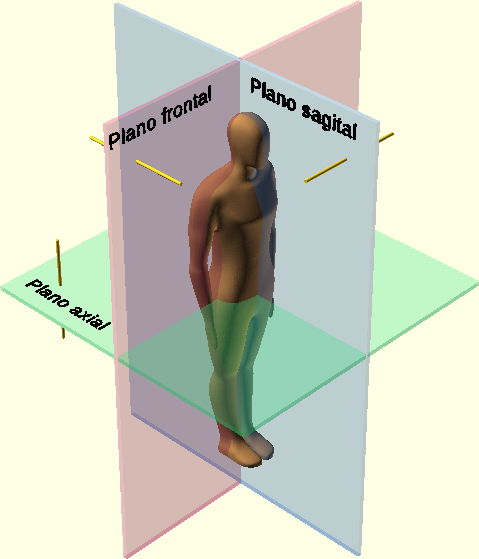
\includegraphics[width=0.55\textwidth]{body-plane/files/body-plane.png}
  \caption{ Planos e eixos no corpo humano.}
\label{fig:bodyhumanplane}
\end{figure}

\begin{definition}[Eixo axial:] 
\index{Eixo axial}
\label{def:EixoAxial}
É o eixo perpendicular ao plano axial.
Ver Figura \ref{fig:bodyhumanplane}.
\end{definition}

\begin{definition}[Eixo frontal:] 
\index{Eixo frontal}
\label{def:EixoFrontal}
É o eixo perpendicular ao plano frontal.
Ver Figura \ref{fig:bodyhumanplane}.
\end{definition}

\begin{definition}[Eixo sagital:] 
\index{Eixo sagital}
\label{def:EixoSagital}
É o eixo perpendicular ao plano sagital.
Ver Figura \ref{fig:bodyhumanplane}.
\end{definition}
%%%%%%%%%%%%%%%%%%%%%%%%%%%%%%%%%%%%%%%%%%%%%%%%%%%%%%%%%%%%%%%%%%%%%%%%%%%%%%%%
\subsection{Definições sobre o abraço nas danças a dois}

\begin{definition}[Firmeza de braços (Dança):]
\index{Firmeza de braços}
\label{def:brazosfirmes} 
Que o \hyperref[def:Condutor]{\textbf{condutor}} e \hyperref[def:Seguidor]{\textbf{seguidor}}
tenham os braços firmes, não implica fazer força pra submeter ao par;
e sim, ativar os músculos o mínimo e necessário para manter a posição relativa dos braços.
de modo que a informação de condução passe através dos braços no abraço, 
e chegue com fidelidade ao corpo do seguidor.

Outra forma de descrever a firmeza dos braços, 
é indicando que esta ação implica ter uma ativação muscular e auto controle, 
para suprimir conscientemente alguns graus de liberdade que existem nas articulações nos braços, 
dependendo da situação e do estilo de dança.
\end{definition}




Na Figura \ref{fig:modelobrazo} podemos ver um modelo simplificado de um braço,
usando 5 graus de liberdade:
\begin{itemize}
\item 2 graus de liberdade, $\theta_1$ e $\theta_2$, nos movimentos de rotação e abertura do ombro.
\item 1 grau de liberdade, $\theta_3$, no movimento de flexão no cotovelo.
\item 1 grau de liberdade, $\theta_4$, no movimento de rotação no antebraço.
\item 1 grau de liberdade, $\theta_5$, no movimento de flexão no pulso.
\end{itemize}

 

\begin{figure}[!ht]
     \centering
     \begin{subfigure}[b]{0.31\textwidth}
         \centering
         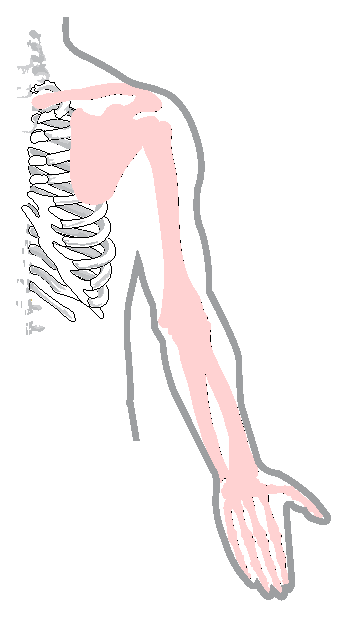
\includegraphics[width=\textwidth]{chapters/cap-normas/brazo1.eps}
         \caption{Modelo humano}
         \label{fig:modelobrazo1}
     \end{subfigure}
     \hfill
     \begin{subfigure}[b]{0.31\textwidth}
         \centering
         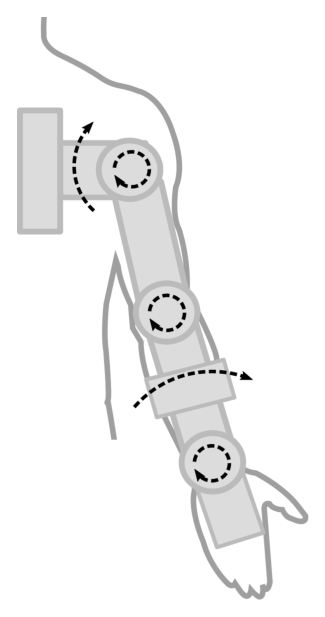
\includegraphics[width=\textwidth]{chapters/cap-normas/brazo2.eps}
         \caption{Modelo mecánico}
         \label{fig:modelobrazo2}
     \end{subfigure}
     \hfill
     \begin{subfigure}[b]{0.31\textwidth}
         \centering
         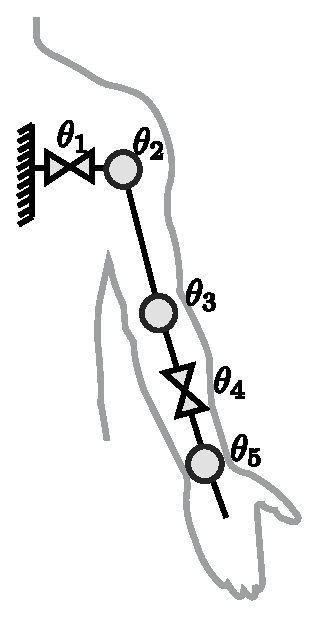
\includegraphics[width=\textwidth]{chapters/cap-normas/brazo3.eps}
         \caption{Modelo teórico}
         \label{fig:modelobrazo3}
     \end{subfigure}
\caption{Modelo de um braço}
\label{fig:modelobrazo}
\end{figure}

Quando iniciamos nosso aprendizado na dança, 
o primeiro grau de liberdade que aprendemos a bloquear de forma inteligente é $\theta_5$ (pulso),
pois é o que instintivamente fazemos quando nos indicam ter os braços firmes.
O grau de liberdade representado por $\theta_4$ (antebraço), geralmente estará livre na nossa dança,
e ajudará a ter uma postura confortável no abraço.
Quando realmente iniciamos a entender, que é ter firmeza do braços,
é quando iniciamos a controlar o grau de liberdade representado por $\theta_3$ (cotovelo);
pois esta articulação permite que nosso par de dança sempre esteja dentro de nosso abraço.
O último nível de nosso aprendizagem para garantir a firmeza de braços,
é controlar consciente e inteligentemente quando bloquear  $\theta_1$ e $\theta_2$ (hombro),
esta articulação é muito descuidada pelos condutores e seguidores,
pois a maioria das pessoas vem como alvo final do seu treinamento,
controlar a articulação do cotovelo. 

\begin{definition}[Abraço de dança:]
\index{Abraço de dança}
\label{def:abracodedanca}  
É um abraço onde o \hyperref[def:Condutor]{\textbf{condutor}} 
rodeia com a mão direita as costas do \hyperref[def:Seguidor]{\textbf{seguidor}},
numa linha meia entre a linha dos ombros e a linha da parte baixa do tórax;
enquanto a mão esquerda, do condutor, segura com o braço semi flexionado a mão direita do seguidor,
colocando ambas mãos a altura do ombro da pessoa mais baixa do \hyperref[def:Par]{\textbf{par}}.
Por outro lado, o seguidor também rodeia com seus braços ao condutor,
de modo que seu braço esquerdo rodeie o braço direto do condutor ate chegar,
na medida do possível, na altura dos ombros. 

É preferível que a palma da mão esquerda do seguidor não esteja apontando ao chão,
para evitar que inconscientemente o seguidor recarregue seu peso no ombro do condutor,
pelo que uma boa alternativa seria que a palma da mão do seguidor aponte a algum ponto no peito do próprio seguidor.

Por motivos similares, é preferível que o cotovelo do braço direito do seguidor,
que segura a mão do condutor,
não aponte ao chão e sim e sim que esteja ligeiramente levantado,
para que não seja esquecido que o peso desse braço ou do corpo não deve ser recarregado no condutor. 
\end{definition}

%%%%%%%%%%%%%%%%%%%%%%%%%%%%%%%%%%%%%%%%%%%%%%%%%%%%%%%%%%%%%%%%%%%%%%%%%%%%%%%%
\subsection{Definições sobre posições corporais  nas danças a dois}


%\textcolor{red}{Postura vs. Posição}

 
\begin{definition}[Posição:] 
\index{Posição}
\label{def:Posicao}O Dicionário Priberam da Língua Portuguesa \cite{priberamposicao} define posição como:
\begin{itemize}
\item Situação de uma coisa.
\item Atitude, postura.
\item Disposição.
\item Circunstâncias em que alguém se acha.
\end{itemize}
Adicionalmente o Dicionário Online de Português, DICIO \cite{dicioposicao}, define princípio como:
\begin{itemize}
\item Postura em que algo ou alguém se coloca ou é colocado
\item Colocação de um corpo em relação a referências externas.
\end{itemize}
\end{definition}


%%%%%%%%%%%%%%%%%%%%%%%%%%%%%%%%%%%%%%%%%%%%%%%%%%%%%%%%%%%%%%%%%%%%%%%%%%%%%%%%
\subsubsection{Classificação seguindo a proximidade dos tórax}

Na Figura \ref{fig:proximidadeabraco1},
podemos ver  3 tipos de posições
para o par dança a dois, 
classificando-os seguindo a proximidade dos torax.
\begin{figure}[!ht]
     \centering
     \begin{subfigure}[b]{0.31\textwidth}
         \centering
         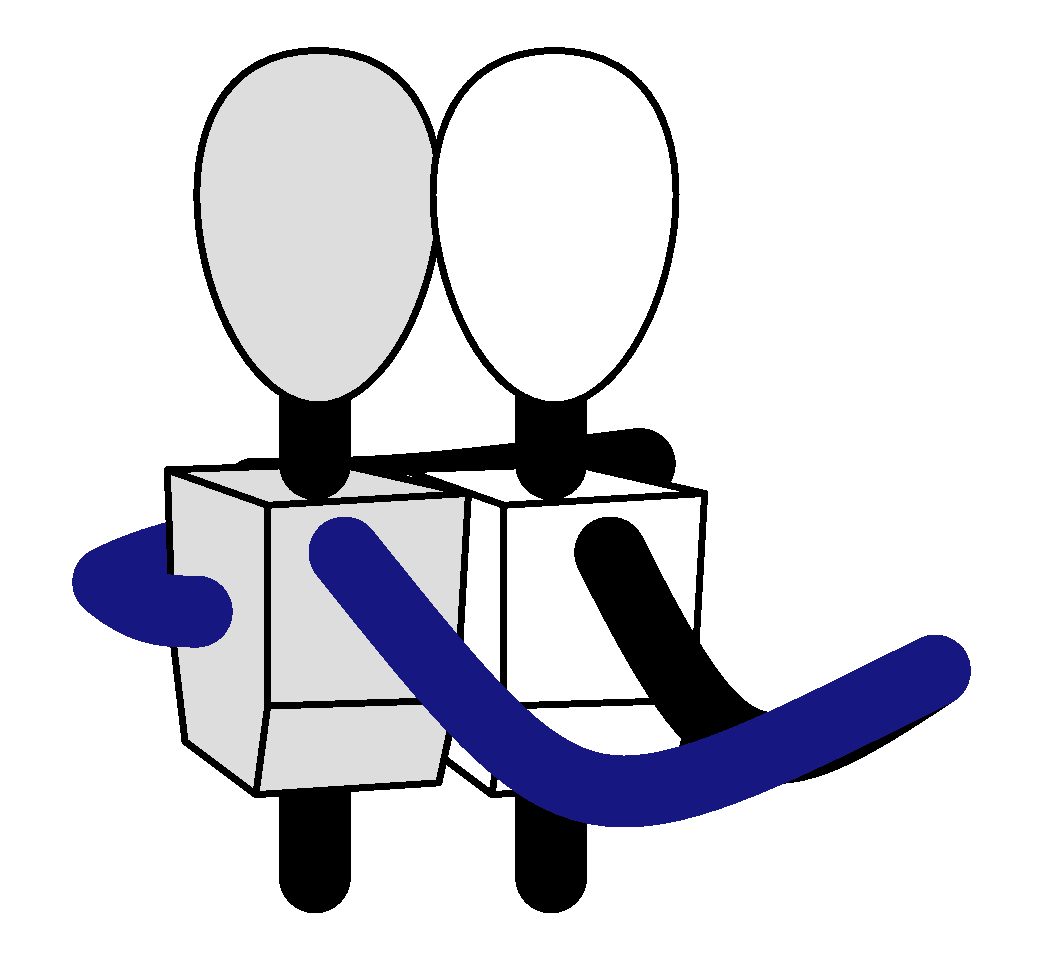
\includegraphics[width=\textwidth]{chapters/cap-normas/position-closed.eps}
         \caption{Posição fechada.}
         \label{fig:proximidadeabraco1:closed}
     \end{subfigure}
     \hfill
     \begin{subfigure}[b]{0.31\textwidth}
         \centering
         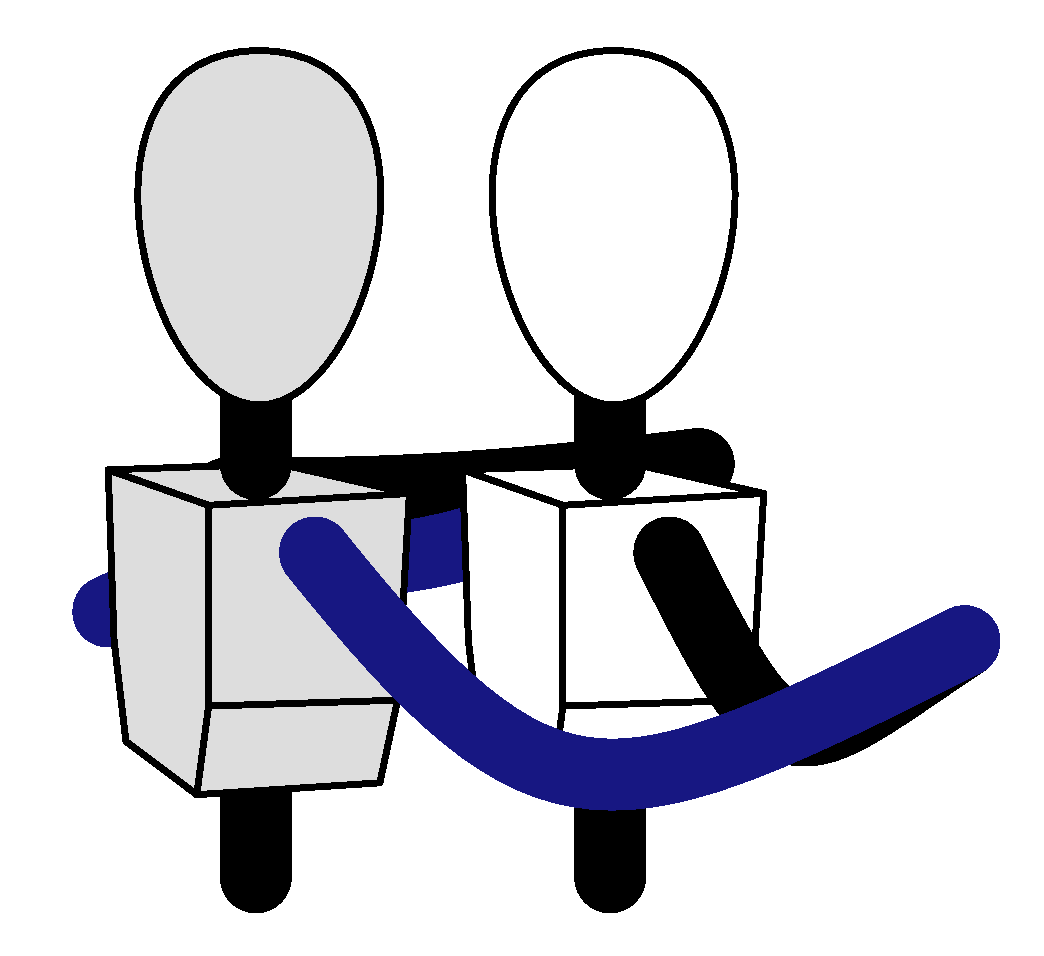
\includegraphics[width=\textwidth]{chapters/cap-normas/position-open.eps}
         \caption{Posição aberta.}
         \label{fig:proximidadeabraco1:open}
     \end{subfigure}
     \hfill
     \begin{subfigure}[b]{0.31\textwidth}
         \centering
         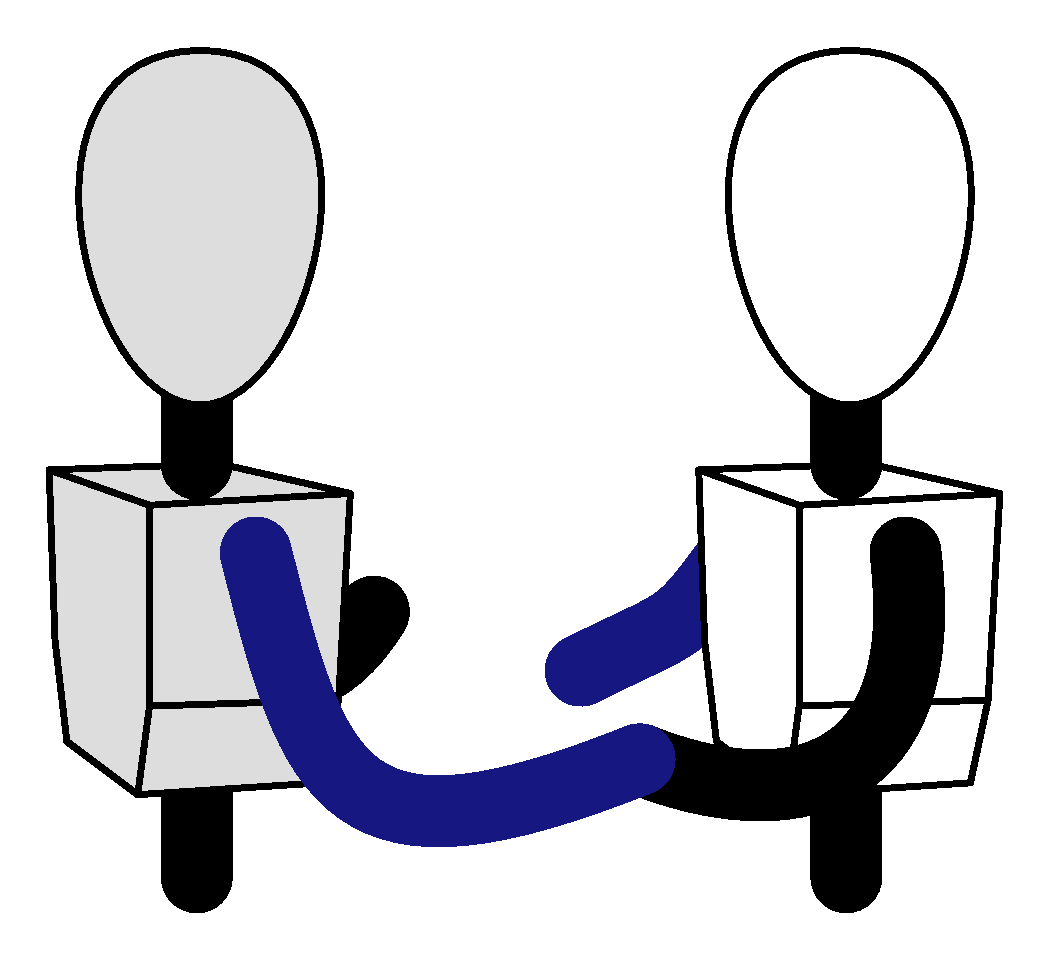
\includegraphics[width=\textwidth]{chapters/cap-normas/position-apart.eps}
         \caption{Posição separada.}
         \label{fig:proximidadeabraco1:apart}
     \end{subfigure}
\caption{Classificação das posições na dança a dois seguindo a proximidade dos corpos.}
\label{fig:proximidadeabraco1}
\end{figure}


\begin{definition}[Posição fechada:]
\index{Posição!Posição fechada}
\label{def:closed-position}  (do inglês ``closed position'')
As pessoas do \hyperref[def:Par]{\textbf{par}} de dança estão frente a frente, tendo contato no tórax,
realizando um \hyperref[def:abracodedanca]{\textbf{abraço de dança}} (ver Figura \ref{fig:proximidadeabraco1:closed}); 
cada pessoa olha por cima do ombro direito do outro,
e os dedos dos pés de cada pessoa apontam a outra \cite{fletsher2015improve} \cite[pp. 6, 8]{harris1998social}.
\end{definition}


\begin{definition}[Posição aberta:]
\index{Posição!Posição aberta}
\label{def:open-position} (do inglês ``open position'') 
É similar à posição fechada, 
com a diferencia que não se tem contanto entre os tórax do \hyperref[def:Par]{\textbf{par}}
(ver Figura \ref{fig:proximidadeabraco1:open}),
estando estes separados, aproximadamente, 1 palmo de distancia \cite{fletsher2015improve} \cite[pp. 8]{harris1998social}.
\end{definition}



\begin{definition}[Posição separada:]
\index{Posição!Posição separada}
\label{def:apart-position} (do inglês ``apart position'' ou ``open facing position'') 
As pessoas do \hyperref[def:Par]{\textbf{par}} de dança estão frente a frente;
porem, elas estão tão separadas (ver Figura \ref{fig:proximidadeabraco1:apart}), 
que não é possível realizar um abraço de dança, 
pelo que o par só se segura por uma ou as duas mãos \cite{fletsher2015improve} \cite[pp. 14]{BallroomDancing1992}.
\end{definition}

%%%%%%%%%%%%%%%%%%%%%%%%%%%%%%%%%%%%%%%%%%%%%%%%%%%%%%%%%%%%%%%%%%%%%%%%%%%%%%%%
\subsubsection{Classificação seguindo o ângulo entre os tórax}
Se classificamos as posições do par de dança seguindo o ângulo entre os tórax,
podemos encontrar a posição fechada, 
a posição promenade e posição lateral, como mostra a Figura \ref{fig:desenhando}.
\begin{figure}[!ht]
     \centering
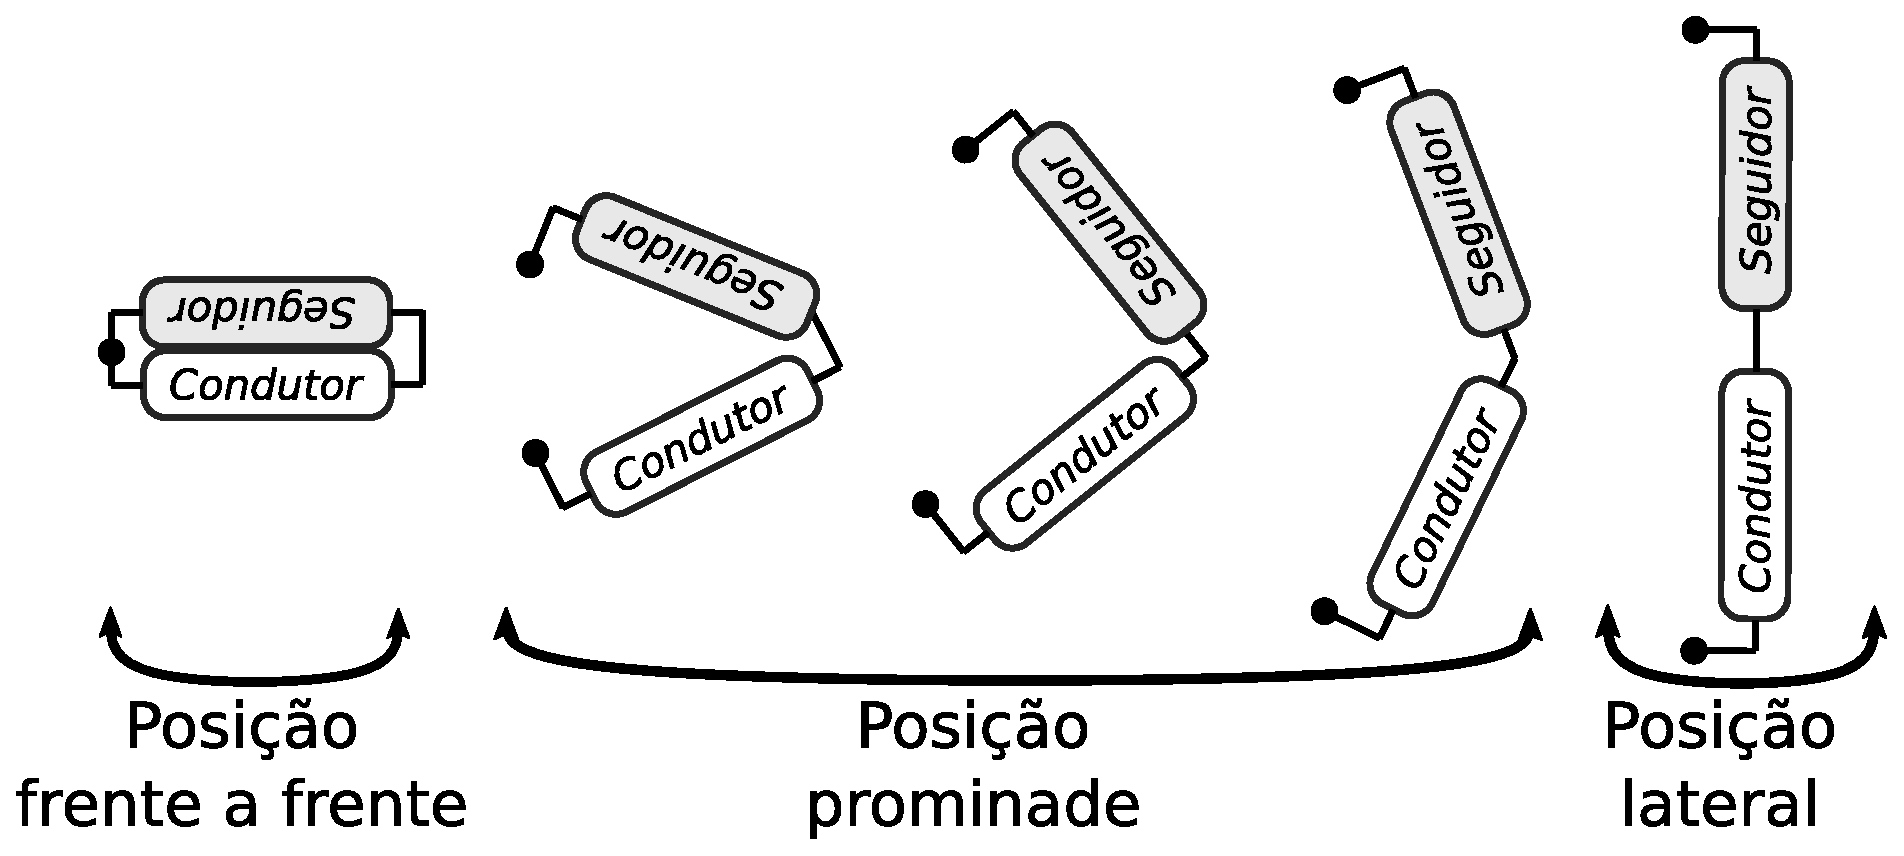
\includegraphics[width=0.81\textwidth]{chapters/cap-normas/desenhando.eps}
\caption{Transição desde a posição frente a frente ate a lateral.}
\label{fig:desenhando}
\end{figure}


\begin{definition}[Posição frente a frente:]
\index{Posição!Posição frente a frente}
\label{def:frente-frente-position} 
Refere-se a uma posição quando ambas pessoas do \hyperref[def:Par]{\textbf{par}}, 
de dança estão com o tórax um frente ao outro,
com as linhas dos tórax do 
\hyperref[def:Condutor]{\textbf{condutor}} e do
\hyperref[def:Seguidor]{\textbf{seguidor}} paralelas.
O abraço de dança pode ter uma posição \hyperref[def:closed-position]{\textbf{fechada}} 
ou \hyperref[def:open-position]{\textbf{aberta}}.
\end{definition}



\begin{definition}[Posição promenade:]
\index{Posição!Posição promenade}
\label{def:promenade-position}  (do inglês ``promenade position'') 
O lado direito do \hyperref[def:Condutor]{\textbf{condutor}} e o 
lado esquerdo do \hyperref[def:Seguidor]{\textbf{seguidor}} estão juntos,
enquanto que o lado esquerdo do condutor e o direito do seguidor estão afastados,
de modo que os tórax, das pessoas do \hyperref[def:Par]{\textbf{par}}, formam um ângulo menor a $180^o$;
é dizer, formam uma posição de V;
eles podem ou não ter as mãos seguradas \cite[pp. 13, 16]{BallroomDancing1992}.
\end{definition}


\begin{definition}[Posição lateral:]
\index{Posição!Posição lateral}
\label{def:lateral-position}  (do inglês ``side position'' ou ``conversation position'') 
O lado direito do \hyperref[def:Condutor]{\textbf{condutor}} e o 
lado esquerdo do \hyperref[def:Seguidor]{\textbf{seguidor}} estão juntos,
enquanto que o lado esquerdo do condutor e o direito do seguidor estão afastados,
de modo que os tórax, das pessoas do \hyperref[def:Par]{\textbf{par}}, formam um ângulo de aproximadamente $180^o$;
eles podem ou não as mãos seguradas \cite{fletsher2015improve} \cite[pp. 8]{harris1998social}.
\end{definition}


%%%%%%%%%%%%%%%%%%%%%%%%%%%%%%%%%%%%%%%%%%%%%%%%%%%%%%%%%%%%%%%%%%%%%%%%%%%%%%%%
\subsubsection{Classificação seguindo a relação estrutural com o par}

Algumas das posições no samba de gafieira tem ganhado nome próprio, 
são mostrados alguns destes casos nas
Figuras \ref{fig:positiongeralsamba:x}, \ref{fig:positiongeralsamba:facao}, 
\ref{fig:positiongeralsamba:facaoinvertido} e \ref{fig:positiongeralsamba:cadeirinha}.
\begin{figure}[!ht]
     \centering
     \begin{subfigure}[b]{0.1805\textwidth}
         \centering
         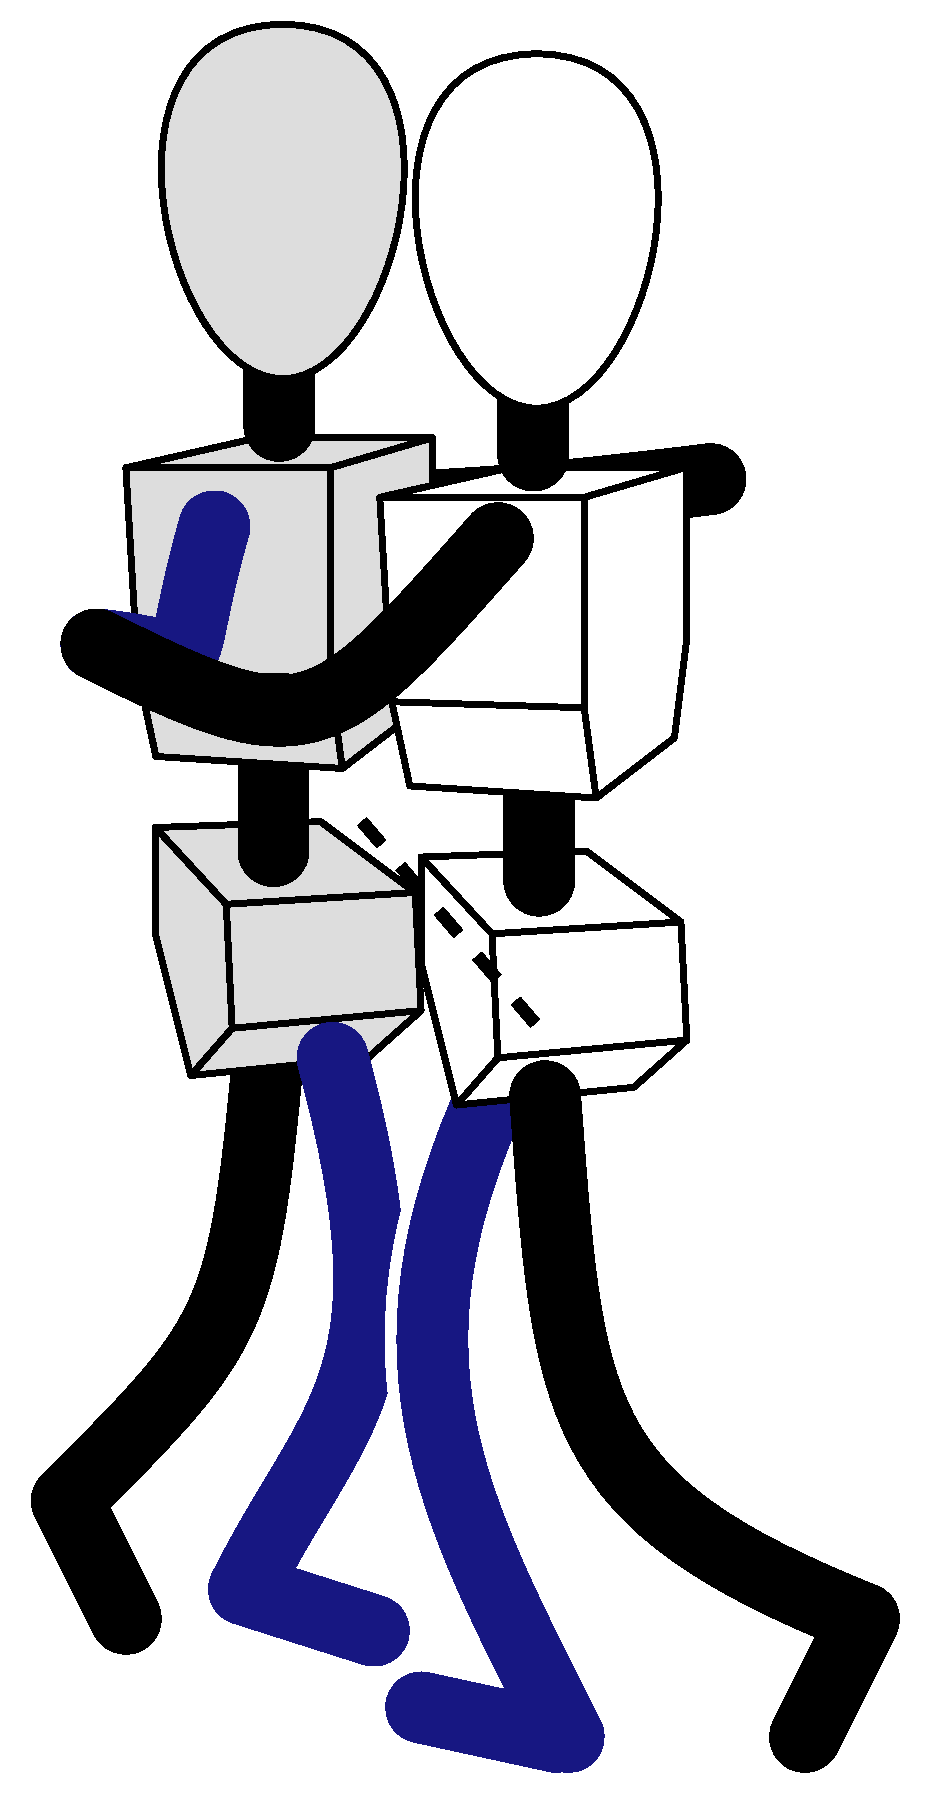
\includegraphics[width=\textwidth]{chapters/cap-normas/position-x.eps}
         \caption{Posição de X.}
         \label{fig:positiongeralsamba:x}
     \end{subfigure}
     \hfill
     \begin{subfigure}[b]{0.19475\textwidth}
         \centering
         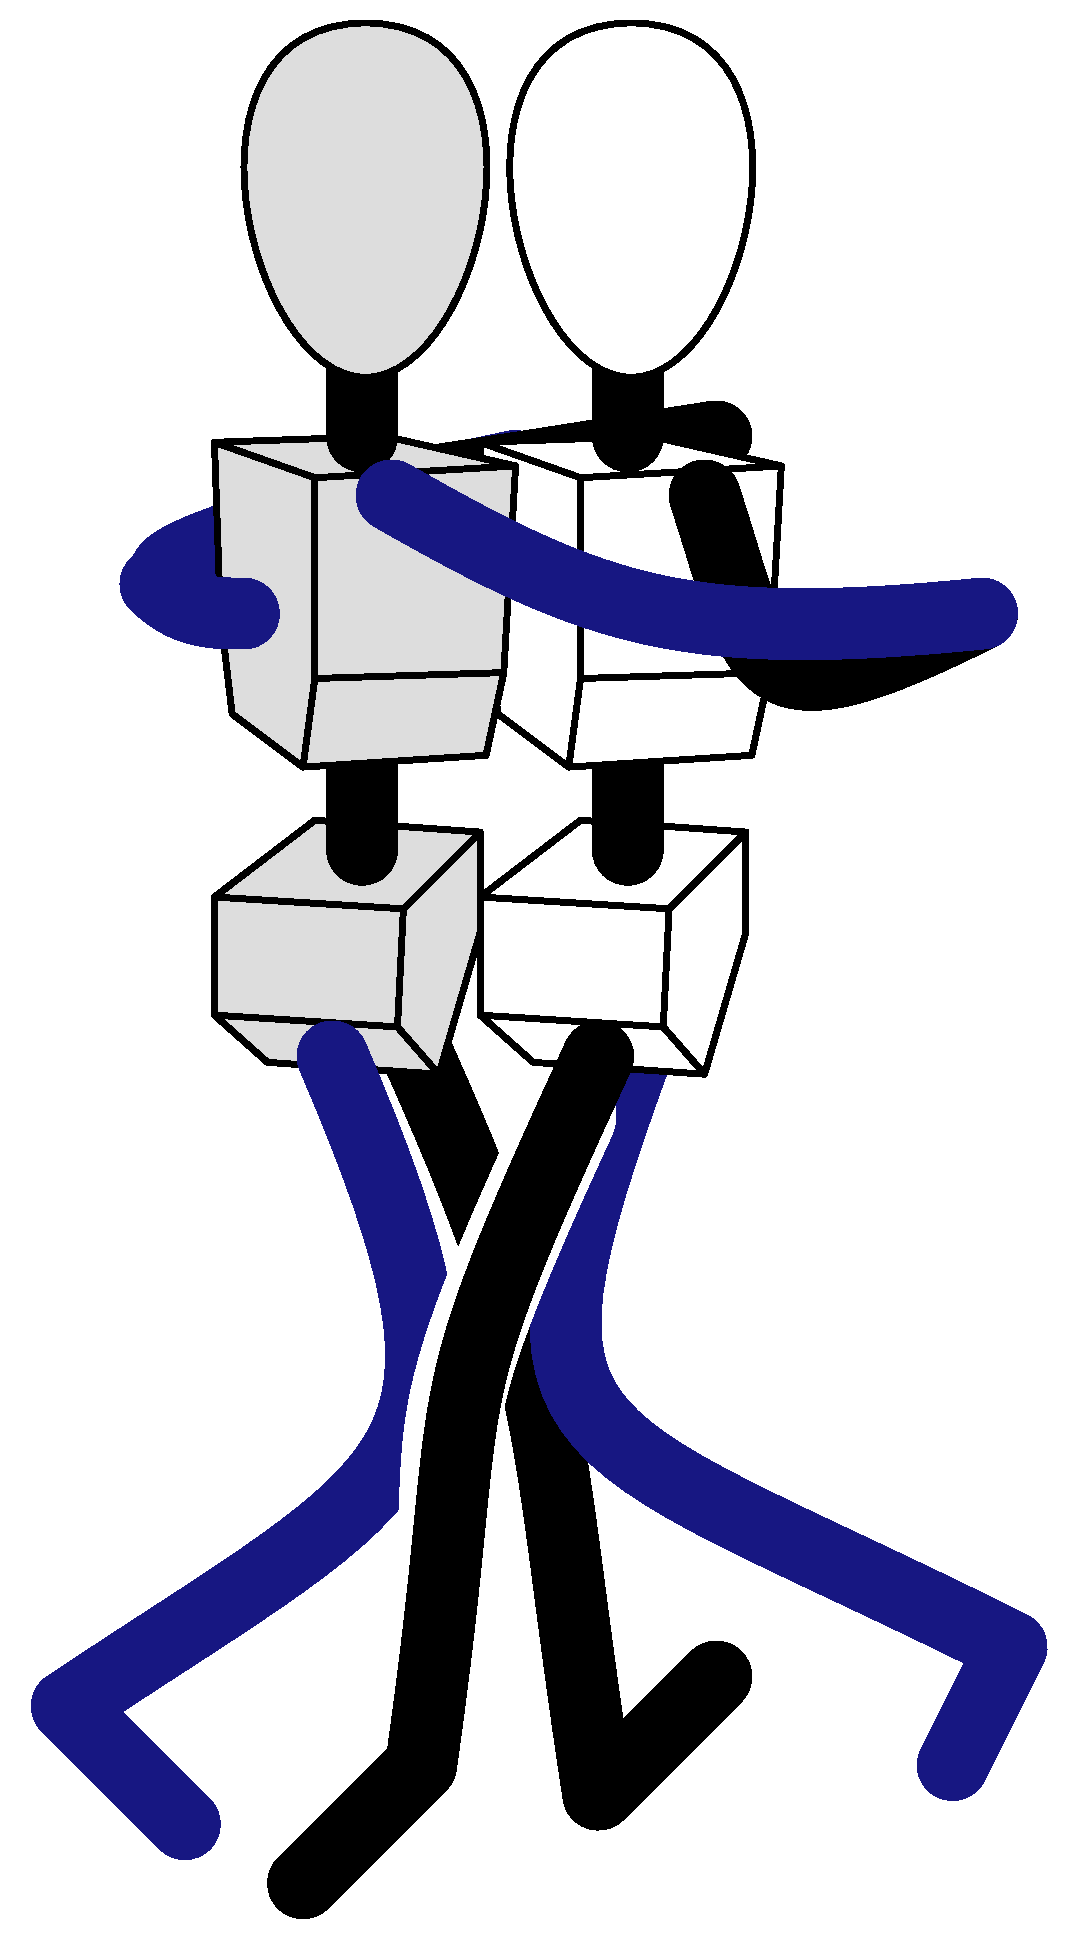
\includegraphics[width=\textwidth]{chapters/cap-normas/position-facao.eps}
         \caption{P. de facão.}
         \label{fig:positiongeralsamba:facao}
     \end{subfigure}
     \hfill
     \begin{subfigure}[b]{0.245\textwidth}
         \centering
         \includegraphics[width=\textwidth]{chapters/cap-normas/position-facao-invertido.eps}
         \caption{P. de facão invertido.}
         \label{fig:positiongeralsamba:facaoinvertido}
     \end{subfigure}
     \hfill
     \begin{subfigure}[b]{0.295\textwidth}
         \centering
         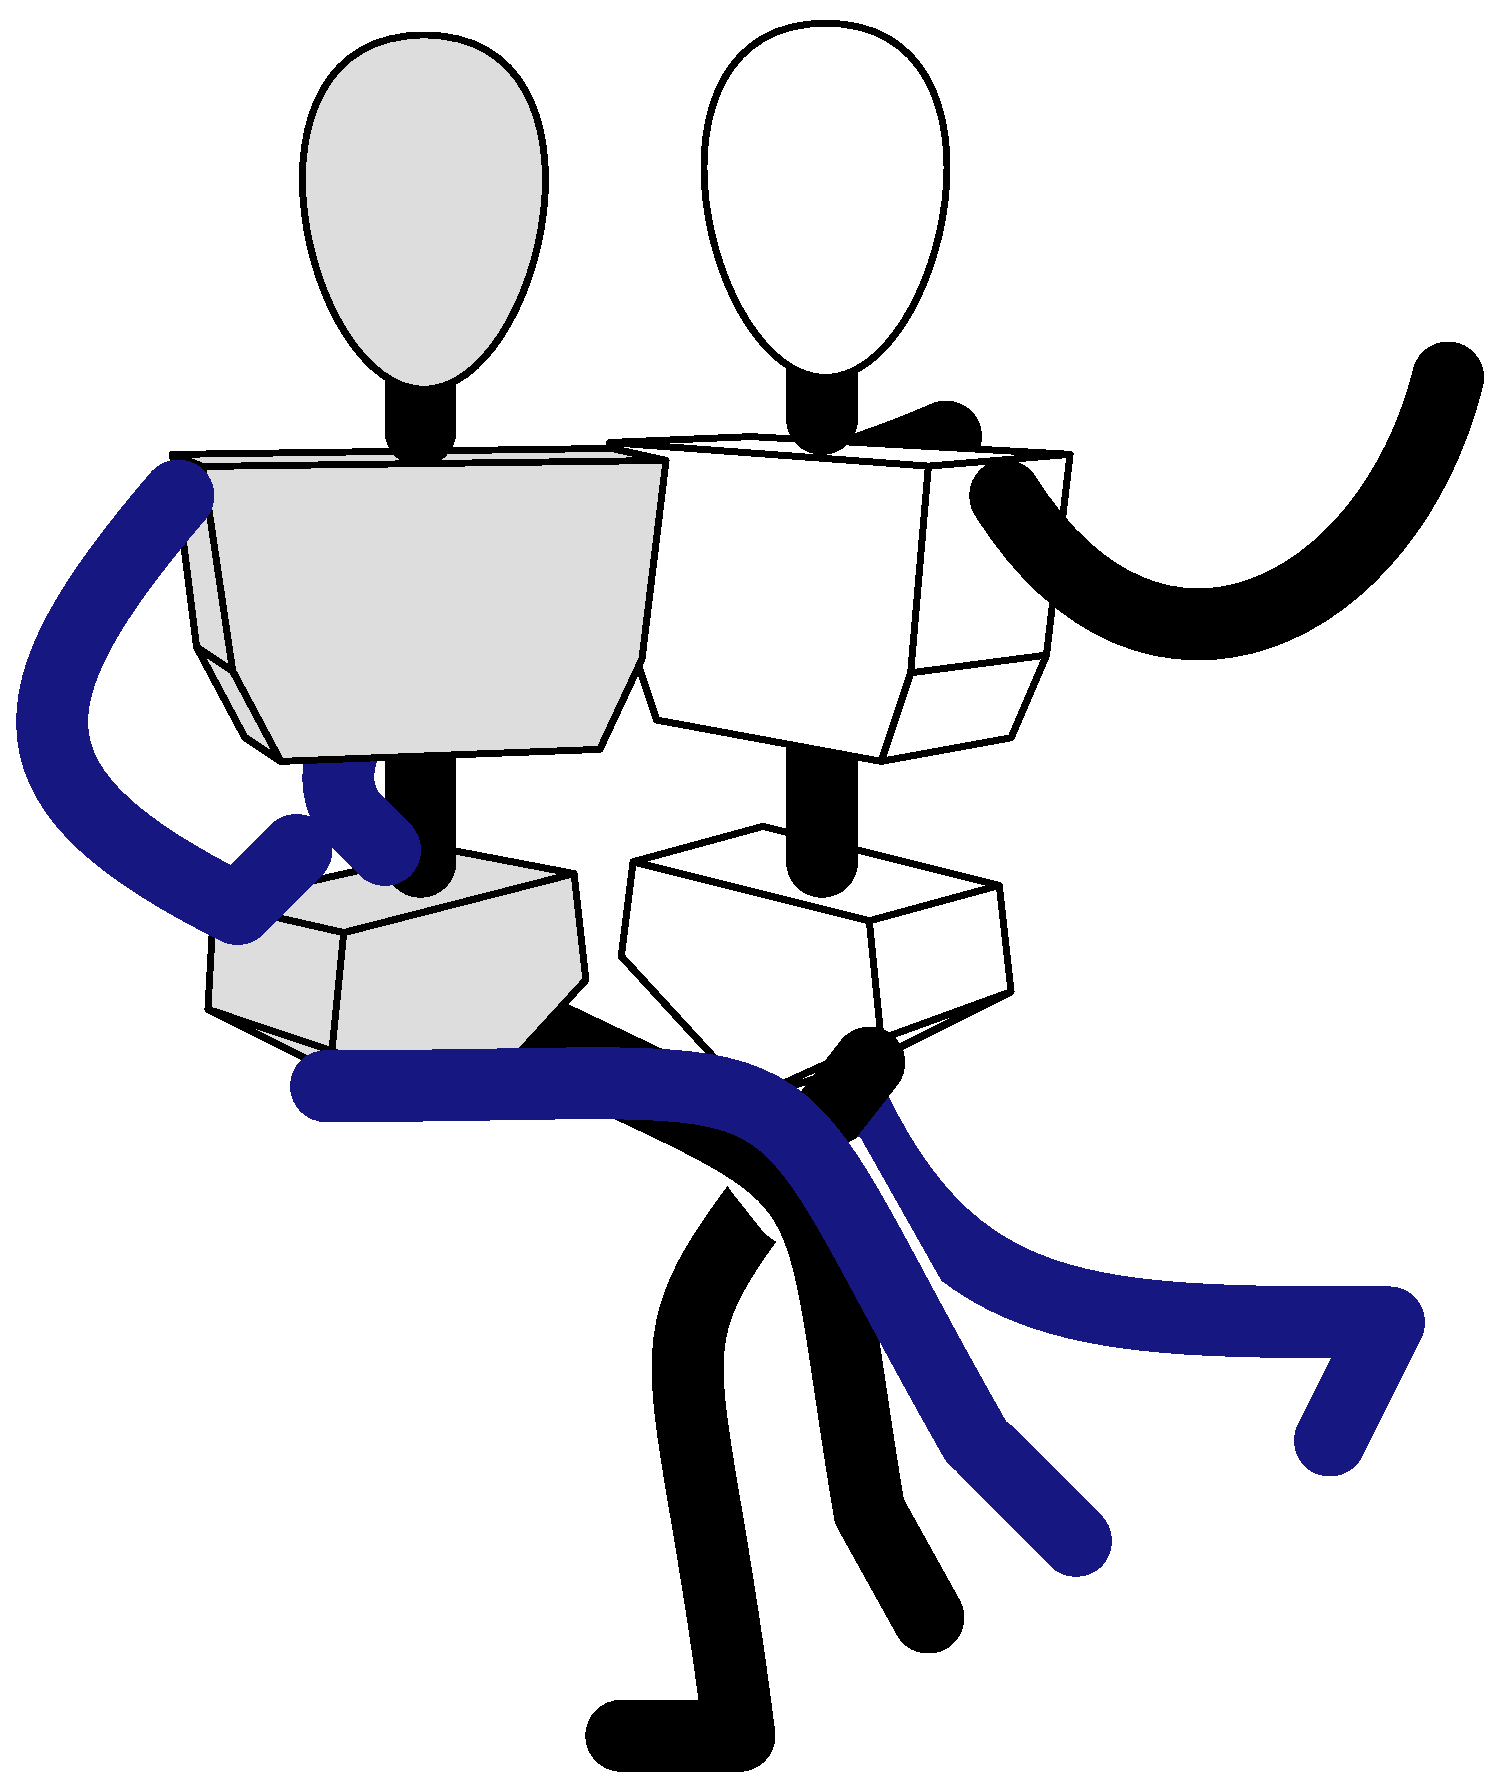
\includegraphics[width=\textwidth]{chapters/cap-normas/position-cadeirinha.eps}
         \caption{Posição de cadeirinha.}
         \label{fig:positiongeralsamba:cadeirinha}
     \end{subfigure}
\caption{Posições comuns no samba de gafieira.}
\label{fig:positiongeralsamba}
\end{figure}

\begin{definition}[Posição de X:]
\index{Posição!Posição de X}
\label{def:X-position} 
Refere-se a uma posição quando ambas pessoas do \hyperref[def:Par]{\textbf{par}} 
de dança estão com o quadril apontando criando linhas paralelas,
o \hyperref[def:Condutor]{\textbf{condutor}} na linha do lado esquerdo e
o \hyperref[def:Seguidor]{\textbf{seguidor}} na linha do lado direito seguindo a Figura \ref{fig:positiongeralsamba:x}.
O par estará formando um \hyperref[def:abracodedanca]{\textbf{abraço de dança}}
que pode ser \hyperref[def:closed-position]{\textbf{fechado}} 
ou \hyperref[def:open-position]{\textbf{aberto}},
sendo que existe dissociação entre o quadril e o tórax;
de modo que os tórax das pessoas do par apontam um ao outro e 
o peso do corpo do condutor está na sua perna direita e do seguidor na perna esquerda (ou dividido).
%As pernas direitas do par formam uma ``X'' em conjunto.
\end{definition}

\begin{definition}[Posição de facão:]
\index{Posição!Posição de facão}
\label{def:facao-position} 
Refere-se a uma posição quando ambas pessoas do \hyperref[def:Par]{\textbf{par}} de dança
estão num \hyperref[def:abracodedanca]{\textbf{abraço de dança}}
em \hyperref[def:closed-position]{\textbf{posição fechada}}.
Cada pessoas do par tem a perna direita para atrás do seu \hyperref[def:PlanoFrontal]{\textbf{plano frontal}},
e a esquerda adiante deste plano, de modo que as poses de ambas pessoas estão
encaixadas sendo estas semelhantes e complementares como mostra a Figura \ref{fig:positiongeralsamba:facao}.
O peso do corpo de ambas pessoas está geralmente dividido entre seus dois pés,
porem distintas distribuições de pesos podem ser usadas.
\end{definition}

\begin{definition}[Posição de facão invertido:]
\index{Posição!Posição de facão invertido}
\label{def:facao-invertido-position} 
Refere-se a uma posição quando ambas pessoas do \hyperref[def:Par]{\textbf{par}} 
de dança estão num \hyperref[def:abracodedanca]{\textbf{abraço de dança}}
em \hyperref[def:promenade-position]{\textbf{posição promenade}}.
As pessoas formam uma ângulo próximo a 90 graus entre seus quadris,
e um menor ângulo na relação do seus tórax, como pode ser visto na Figura \ref{fig:positiongeralsamba:facaoinvertido}.
A perna direita do \hyperref[def:Condutor]{\textbf{condutor}} tem o peso do seu corpo e 
cruza pela frente de sua perna esquerda, fazendo uma leve flexão e com o pé apontando,
na medida do possível, ao \hyperref[def:Seguidor]{\textbf{seguidor}}.
\end{definition}

\begin{definition}[Posição de cadeirinha:]
\index{Posição!Posição de cadeirinha}
\label{def:cadeirinha-position} 
Refere-se a uma posição quando o \hyperref[def:Seguidor]{\textbf{seguidor}} 
está sentado sobre uma das pernas do \hyperref[def:Condutor]{\textbf{condutor}},
tradicionalmente a perna esquerda, como mostra a Figura \ref{fig:positiongeralsamba:cadeirinha}.
O \hyperref[def:abracodedanca]{\textbf{abraço de dança}} pode ter 
uma \hyperref[def:open-position]{\textbf{posição aberta}} e 
\hyperref[def:promenade-position]{\textbf{promenade}}
ou uma  \hyperref[def:lateral-position]{\textbf{posição lateral}}.
\end{definition}

Algumas outras posições no samba de gafieira são muito usadas;
porém estas não tem ganhado nome próprio;
alguns destes  são mostrados nas
Figuras \ref{fig:positiongeralsamba} e \ref{fig:positiongeralsamba:xinvertido}.
\begin{figure}[!ht]
     \centering
     \begin{subfigure}[b]{0.2175\textwidth}
         \centering
         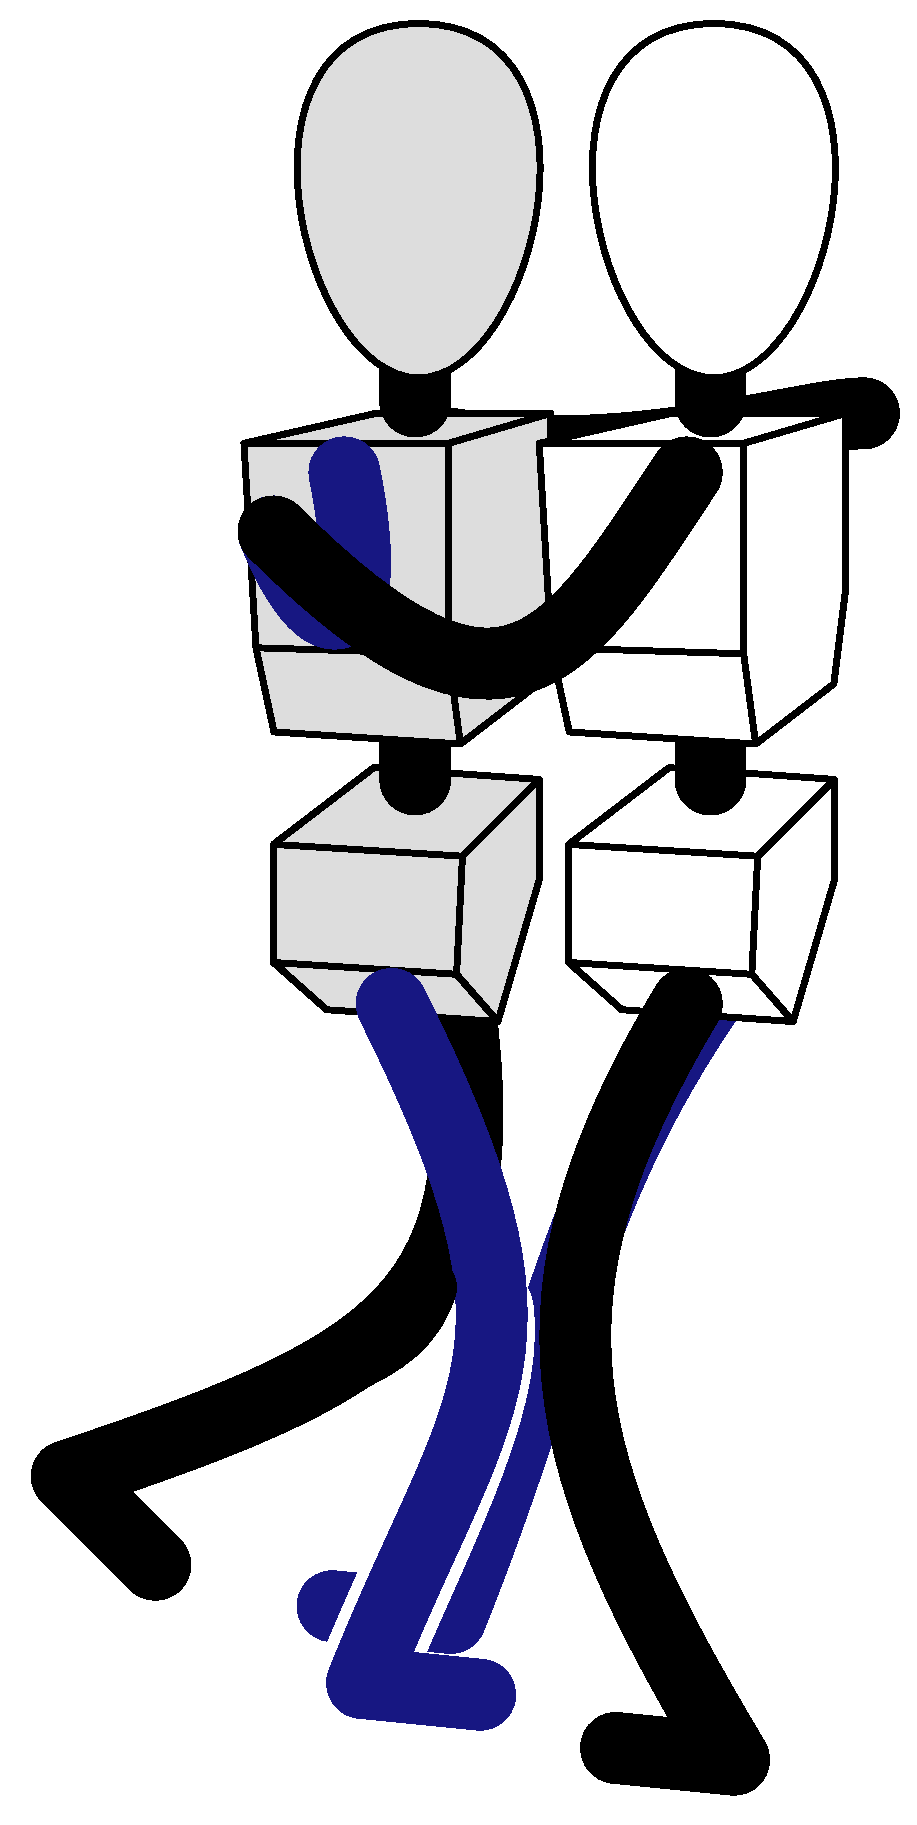
\includegraphics[width=\textwidth]{chapters/cap-normas/position-ffa.eps}
         \caption{Posição frente a frente - atrás.}
         \label{fig:positiongeralsamba:ffa}
     \end{subfigure}
     \hfill
     \begin{subfigure}[b]{0.20\textwidth}
         \centering
         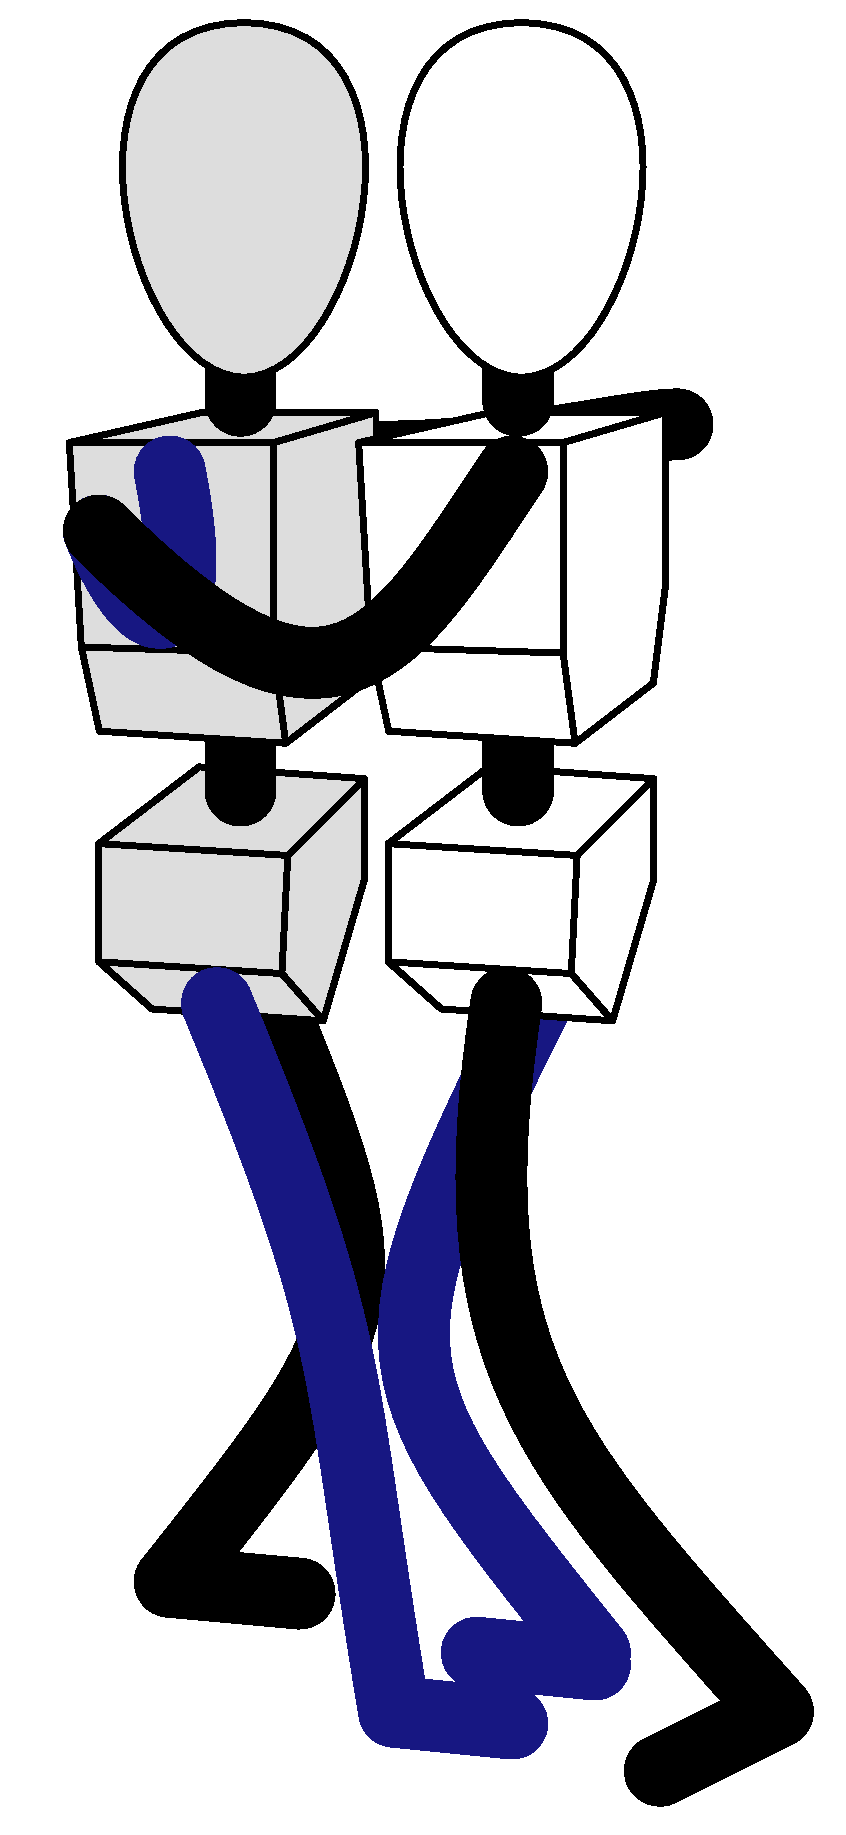
\includegraphics[width=\textwidth]{chapters/cap-normas/position-fff.eps}
         \caption{Posição frente a frente - frente.}
         \label{fig:positiongeralsamba:fff}
     \end{subfigure}
     \hfill
     \begin{subfigure}[b]{0.245\textwidth}
         \centering
         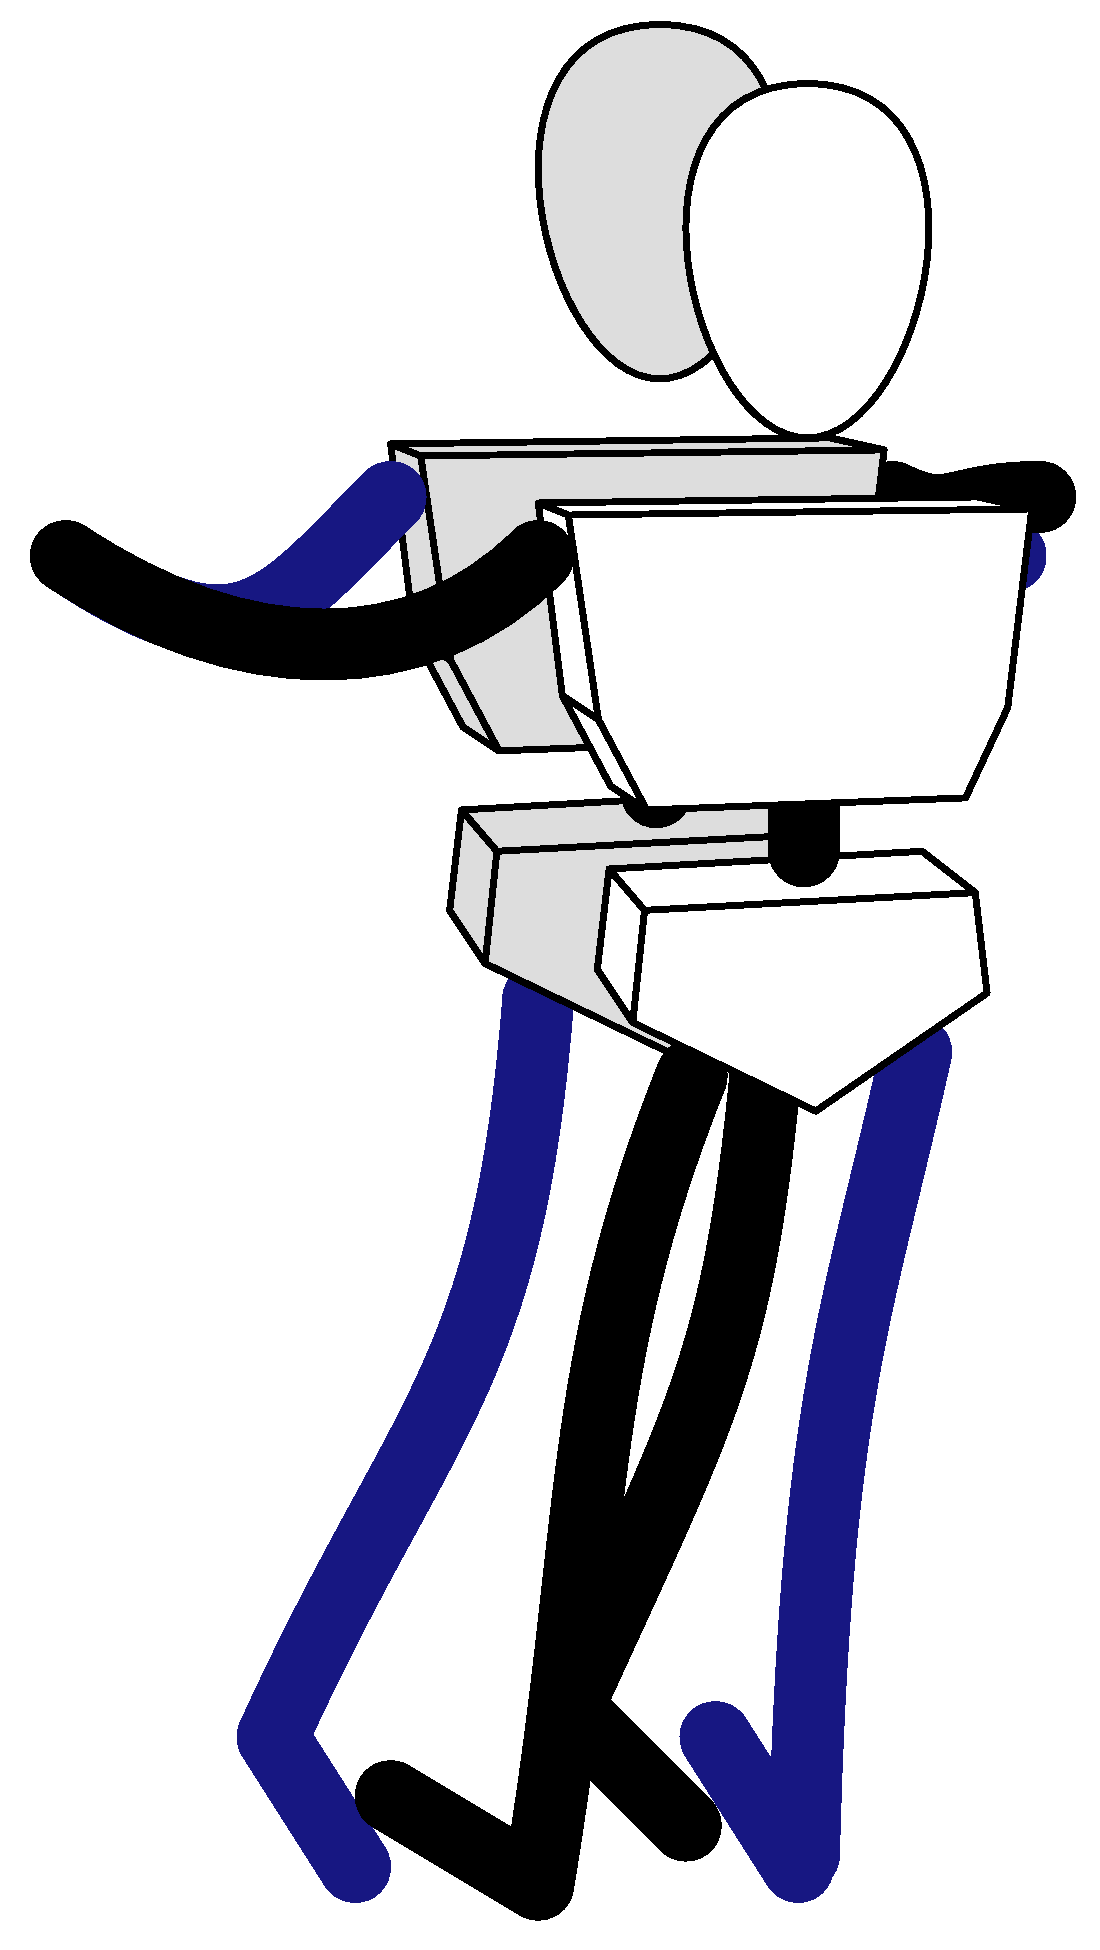
\includegraphics[width=\textwidth]{chapters/cap-normas/position-ffd.eps}
         \caption{Posição frente a frente - direita.}
         \label{fig:positiongeralsamba:ffd}
     \end{subfigure}
     \hfill
     \begin{subfigure}[b]{0.285\textwidth}
         \centering
         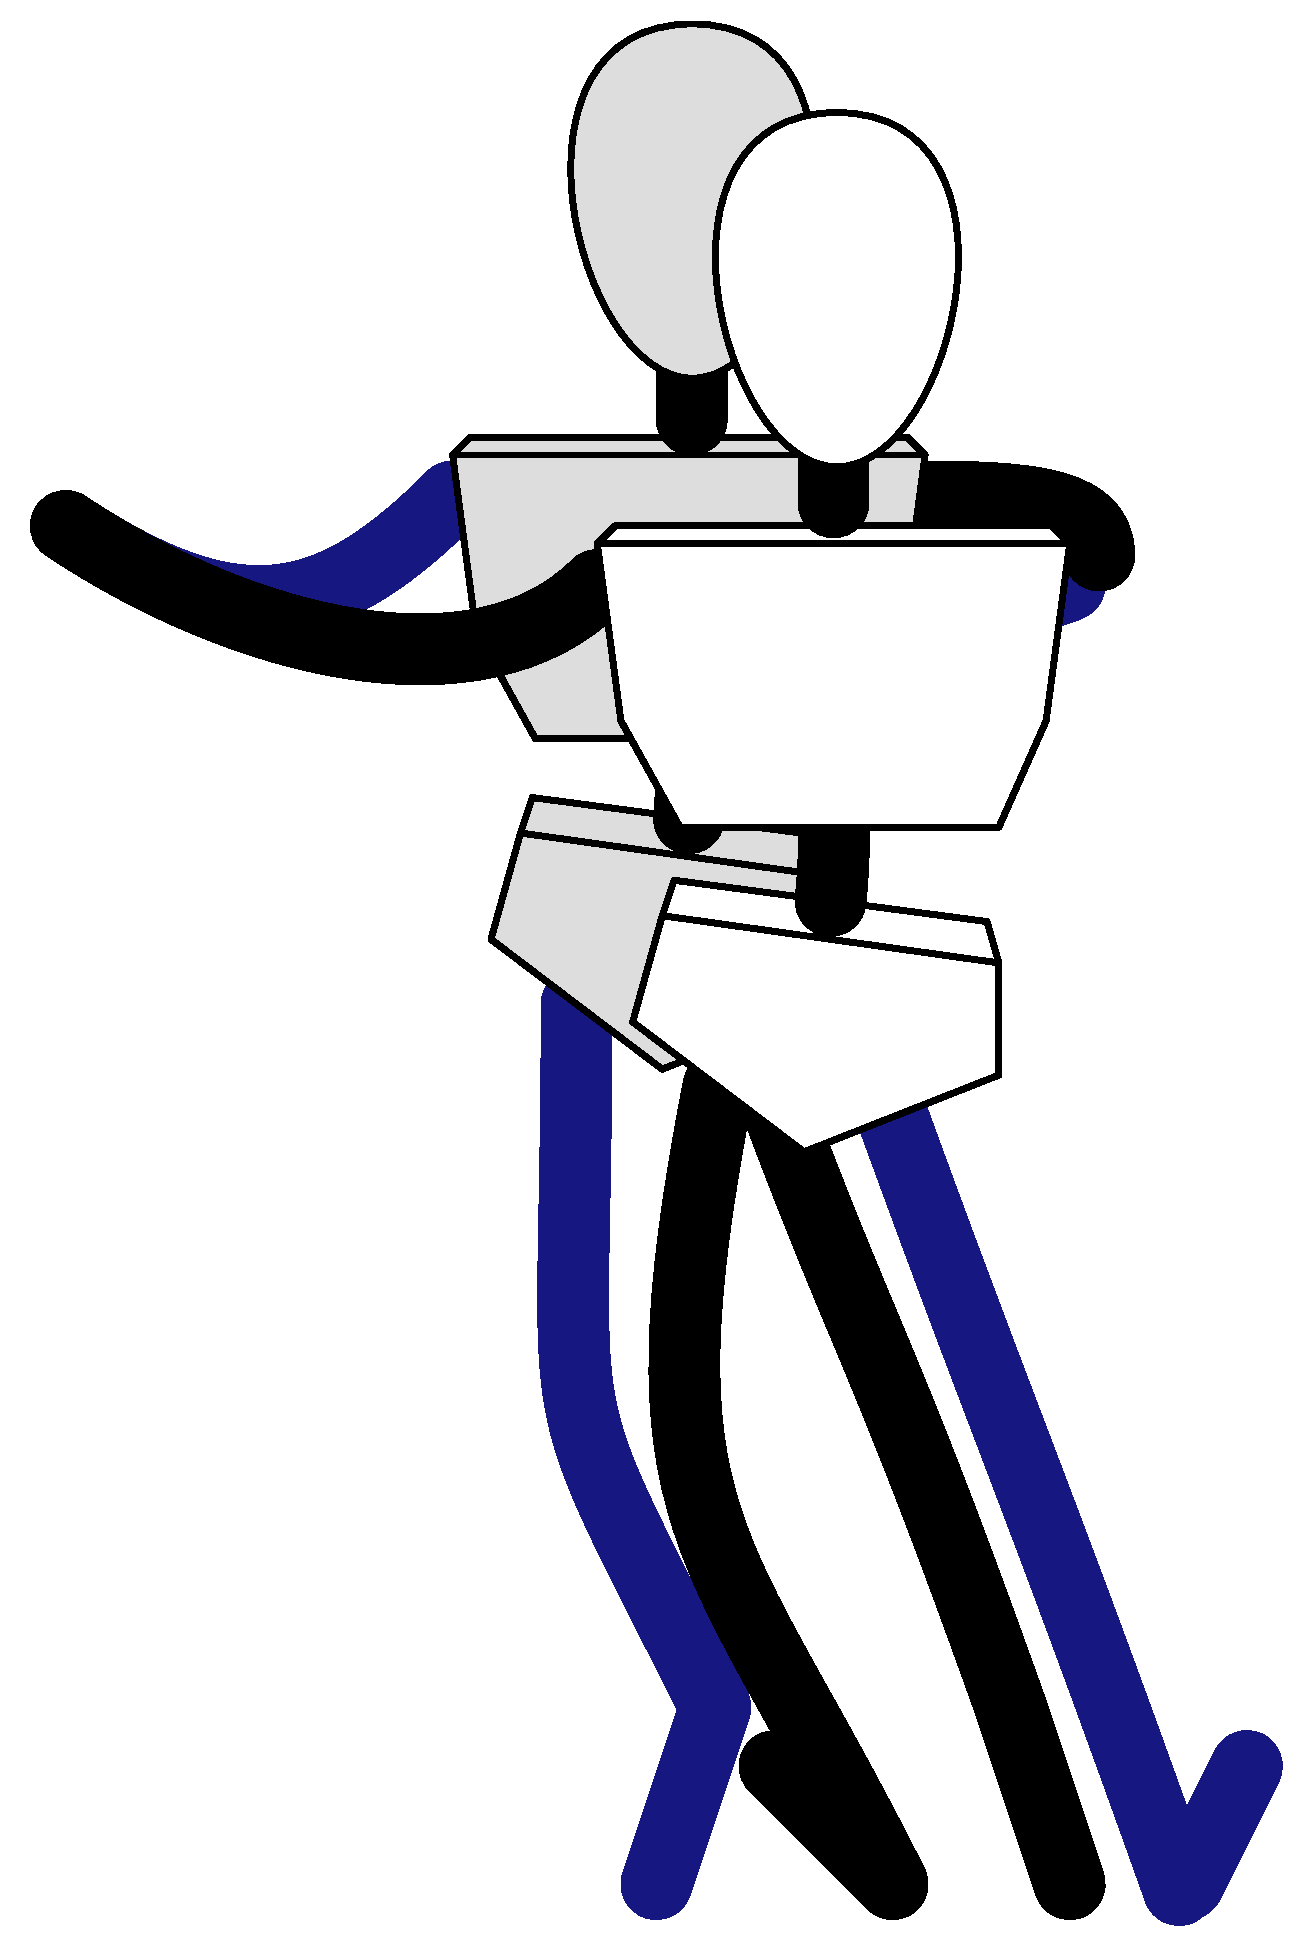
\includegraphics[width=\textwidth]{chapters/cap-normas/position-ffe.eps}
         \caption{Posição frente a frente - esquerda.}
         \label{fig:positiongeralsamba:ffe}
     \end{subfigure}
\caption{Posições comuns no samba de gafieira.}
\label{fig:positiongeralsamba:2}
\end{figure}



\begin{definition}[Posição frente a frente - atrás:]
\index{Posição!Posição frente a frente - atrás}
\label{def:ffa-position}  
Refere-se a uma posição quando ambas pessoas do \hyperref[def:Par]{\textbf{par}}, 
de dança estão com os tórax um frente ao outro, 
como na \hyperref[def:frente-frente-position]{\textbf{posição frente a frente}},
com o detalhe que os pés estão numa posição como indica a Figura \ref{fig:positiongeralsamba:ffa}.
O pé esquerdo do \hyperref[def:Condutor]{\textbf{condutor}} e 
o pé direito do \hyperref[def:Seguidor]{\textbf{seguidor}} levam o peso do corpo,
estando estes colocados para atrás e para adiante do seus \hyperref[def:PlanoFrontal]{\textbf{planos frontais}}, 
respetivamente.
\end{definition}

\begin{definition}[Posição frente a frente - frente:]
\index{Posição!Posição frente a frente - frente}
\label{def:fff-position}  
Refere-se a uma posição quando ambas pessoas do \hyperref[def:Par]{\textbf{par}}, 
de dança estão com os tórax um frente ao outro, 
como na \hyperref[def:frente-frente-position]{\textbf{posição frente a frente}},
com o detalhe que os pés estão numa posição como indica a Figura \ref{fig:positiongeralsamba:fff}.
O pé direito do \hyperref[def:Condutor]{\textbf{condutor}} e 
o pé esquerdo do \hyperref[def:Seguidor]{\textbf{seguidor}} levam o peso do corpo,
estando estes colocados para adiante e para atrás do seus \hyperref[def:PlanoFrontal]{\textbf{planos frontais}}, 
respetivamente.
\end{definition}

\begin{definition}[Posição frente a frente - direita:]
\index{Posição!Posição frente a frente - direita}
\label{def:ffd-position}  
Refere-se a uma posição quando ambas pessoas do \hyperref[def:Par]{\textbf{par}}, 
de dança estão com os tórax um frente ao outro, 
como na \hyperref[def:frente-frente-position]{\textbf{posição frente a frente}},
com o detalhe que os pés estão numa posição como indica a Figura \ref{fig:positiongeralsamba:ffd}.
O pé direito do \hyperref[def:Condutor]{\textbf{condutor}} e 
o pé esquerdo do \hyperref[def:Seguidor]{\textbf{seguidor}} levam o peso do corpo,
com a linha do seus pés paralela ao \hyperref[def:PlanoFrontal]{\textbf{plano frontai}}.
\end{definition}


\begin{definition}[Posição frente a frente - esquerda:]
\index{Posição!Posição frente a frente - esquerda}
\label{def:ffe-position}  
Refere-se a uma posição quando ambas pessoas do \hyperref[def:Par]{\textbf{par}}, 
de dança estão com os tórax um frente ao outro, 
como na \hyperref[def:frente-frente-position]{\textbf{posição frente a frente}},
com o detalhe que os pés estão numa posição como indica a Figura \ref{fig:positiongeralsamba:ffe}.
O pé esquerdo do \hyperref[def:Condutor]{\textbf{condutor}} e 
o pé direito do \hyperref[def:Seguidor]{\textbf{seguidor}} levam o peso do corpo,
com a linha do seus pés paralela ao \hyperref[def:PlanoFrontal]{\textbf{plano frontai}}.
\end{definition}


\begin{definition}[Posição de X invertido:]
\index{Posição!Posição de X invertido}
\label{def:X-invertido-position} 
Refere-se a uma posição quando ambas pessoas do \hyperref[def:Par]{\textbf{par}} 
de dança estão com o quadril apontando criando linhas paralelas,
o \hyperref[def:Condutor]{\textbf{condutor}} na linha do lado esquerdo e
o \hyperref[def:Seguidor]{\textbf{seguidor}} na linha do lado direito seguindo a Figura \ref{fig:positiongeralsamba:xinvertido}.
O par estará formando um \hyperref[def:abracodedanca]{\textbf{abraço de dança}}
que pode ser \hyperref[def:closed-position]{\textbf{fechado}} 
ou \hyperref[def:open-position]{\textbf{aberto}},
sendo que existe dissociação entre o quadril e o tórax;
de modo que os tórax das pessoas do par apontam um ao outro e 
o peso do corpo do condutor está na sua perna esquerda e do seguidor na perna direita (ou dividido).
\end{definition}

\begin{figure}[!ht]
         \centering
         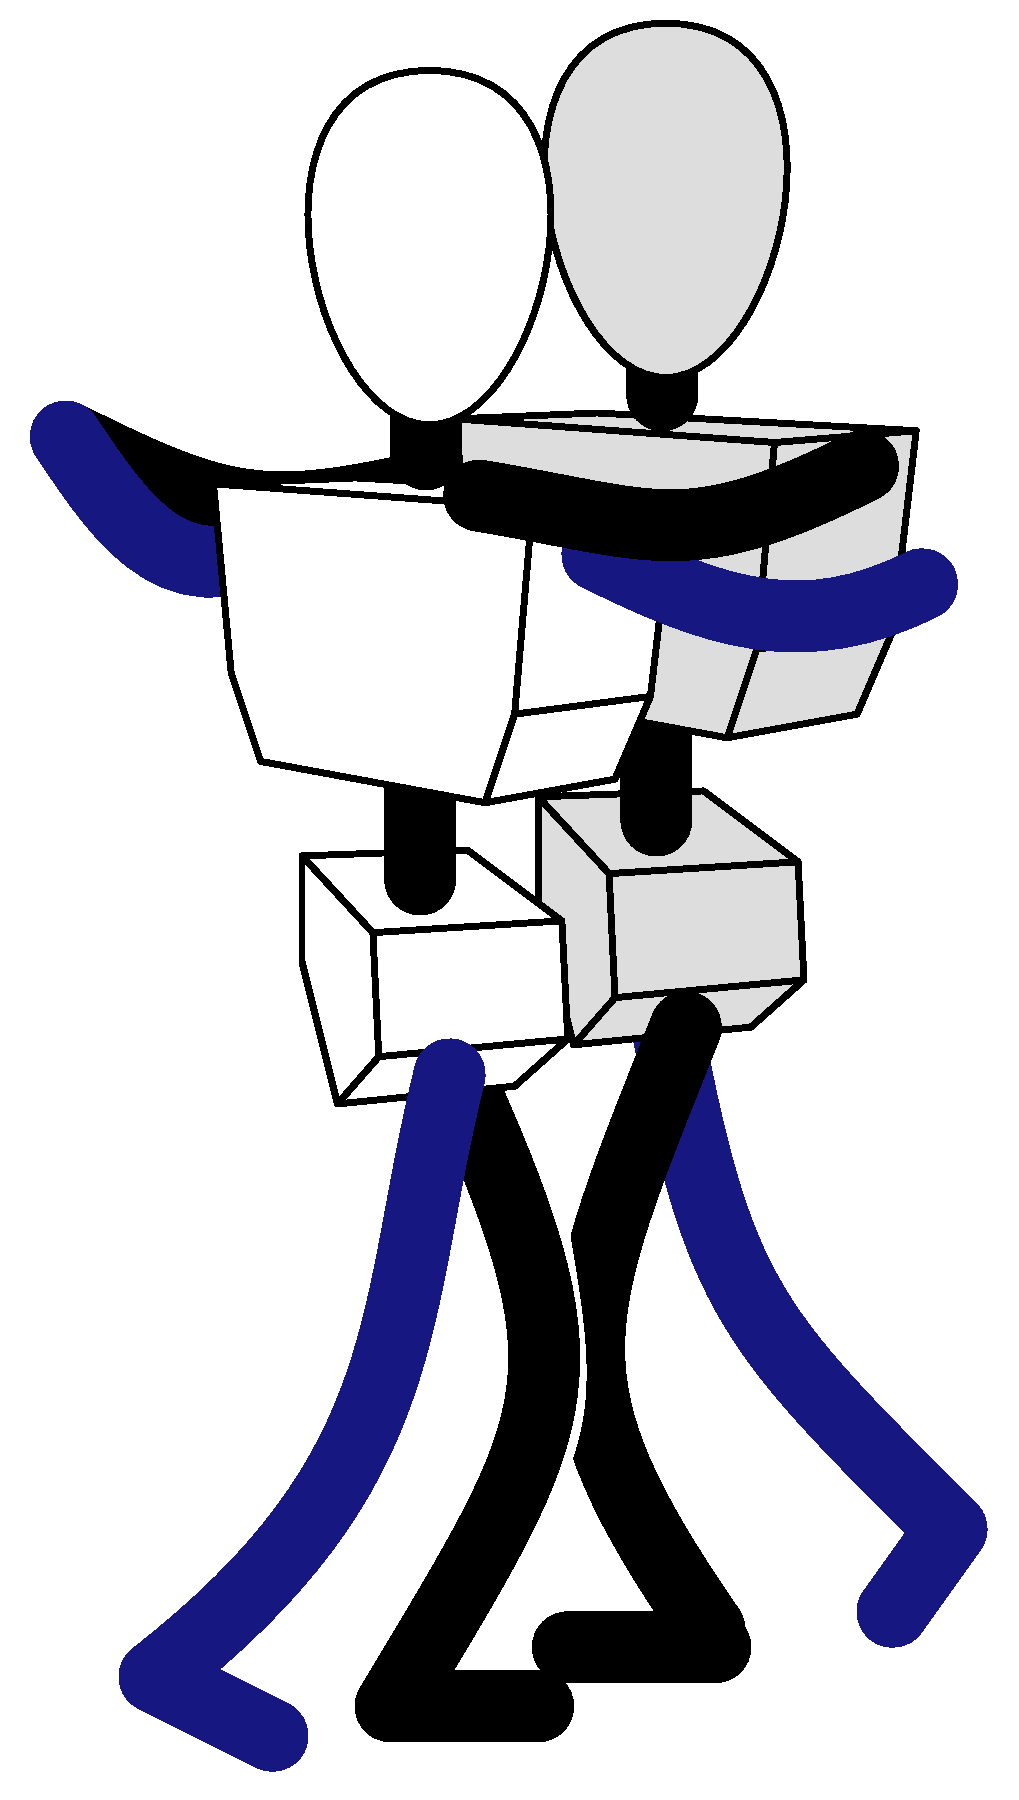
\includegraphics[width=0.21\textwidth]{chapters/cap-normas/position-x-inverso.eps}
         \caption{Posição de X invertido.}
         \label{fig:positiongeralsamba:xinvertido}
\end{figure}

%%%%%%%%%%%%%%%%%%%%%%%%%%%%%%%%%%%%%%%%%%%%%%%%%%%%%%%%%%%%%%%%%%%%%%%%%%%%%%%%
\subsection{Definições sobre modos de dançar em função do tempo musical usado como guia}



\begin{definition}[Dançar no tempo forte:] 
\index{Dançar no tempo forte}
\label{def:DancaNoTempo}
Ou simplesmente \textbf{dançar no tempo}, indica que se está dançando com passos com o movimento principal 
(ou inicial dependendo do ponto de vista ou o estilo de dança), 
se executando no tempo forte da música; ver Exemplo \ref{example:dancatempoforte}.
\end{definition}
\begin{example}
\label{example:dancatempoforte}
Se definimos um passo de dança como: Pisar, usando um pé cada vez, 
realizando um movimento com uma distribuição espacial, junto-junto-longo;
e definimos ao movimento ``longo'' como o movimento principal. 
Se executássemos o movimento ``longo'' no tempo forte, o passo junto-junto-longo,
estaria sendo dançado no tempo forte.
\end{example}

\begin{definition}[Dançar em contra do tempo forte:] 
\index{Dançar em contra do tempo forte}
\label{def:DancaNoContratempo}
Indica que se está dançando, com o movimento principal\footnote{Geralmente o movimento inicial é o principal,
porem depende do estilo de dança.} do passo, 
executando-se em contra do tempo forte da música; é dizer, 
executando-se acentuando um tempo fraco da música (em \hyperref[sec:contratempo]{\textbf{contratempo}}).
A diferencia de \hyperref[def:DancaNoTempo]{\textbf{dançar no tempo forte}}, 
que tem um único modo, pois só existe um tempo forte;
existem varias formas de dançar em contra do tempo forte;
é dizer, como o movimento principal em algum tempo fraco; ver Exemplo \ref{example:dancatempofraco}.
\end{definition}
\begin{example}
\label{example:dancatempofraco}
Se definimos um passo de dança como: Pisar, usando um pé cada vez, 
realizando um movimento com uma distribuição espacial, junto-junto-longo;
e definimos ao primeiro movimento ``junto'' como o movimento principal. 
Se executássemos o movimento ``longo'' no tempo forte, o passo junto-junto-longo,
estaria sendo dançado em contra do tempo forte.
\end{example}
